\chapter{Results and Discussion}

\section{SCAN vs. r$^2$SCAN}
Strongly Constrained and Appropriately Normed Semilocal Density Functional
(SCAN) is  a nonempirical semilocal meta-GGA functional that satisfies all
known possible 17 exact constraints and  appropriately normed on systems for
which semilocal functionals can be exact or extremely accurate
~\cite{sun2015strongly}.  SCAN is not fitted to any bonded system, but it
predicts certain bonding properties very well such as  atomization
energies, weak-interaction binding energies, and lattice
constants of solids, but not the energy barriers to chemical
reactions. It was shown that SCAN accurately describes covalent bonds, hydrogen
bonds, and van der Waals interactions that plays important role in the
structure and dynamics of liquid water~\cite{chen2017ab}. It is one of the
functionals that predicts ice as less dense than liquid water under standard
conditions. Unfortunately,
imposing rigid constraints can cause numerical instabilities for which we have
observed when applying SCAN for systems with interfaces. Instead, this study
used an accurate and numerically efficient regularized-restored r$^2$SCAN
meta-generalized gradient
approximation \cite{Furness2020}. r$^2$SCAN functional satisfies the most
important exact constraints but with more consistent error with grid density,
requiring smaller
grids to
achieve good accuracy.

We performed a comparison between SCAN	and r$^2$SCAN exchange-correlation
functional. Convergence tests were conducted to determine the appropriate
energy cut-offs for the DFT calculations. As shown in
Figures~\ref{fig:conv_scan} and \ref{fig:conv_r2scan}, a  cutoff of 130 Ry  is
adequate to have convergence on  energy, force, and pressure for both the SCAN
and r$^2$SCAN functional. This is also consistent to what Chen et al. used in
their modelling of water \cite{chen2017ab}. Figure~\ref{fig:scan_r2scan_E}
shows that the energy is
underestimated systematically for the r$^2$SCAN functional. Meanwhile,
Figure~\ref{fig:scan_r2scan_F} shows good agreement of the forces between the
two functionals. We computed the root mean square error of the two forces to be
0.0484 \unit{eV/\angstrom}, which is on the same magnitude as typical
validation
errors
on ML models. See Figure~\ref{fig:scan_r2scan_F_dist} for the distribution
plot of the error in forces. For the pressure tensor, it is again
underestimated for r$^2$SCAN functional with respect to the SCAN functional as
verified in  Figure~\ref{fig:scan_r2scan_P}.
\begin{figure}[tbhp]
  \centering
  \begin{subfigure}{0.48\textwidth}
    \centering

    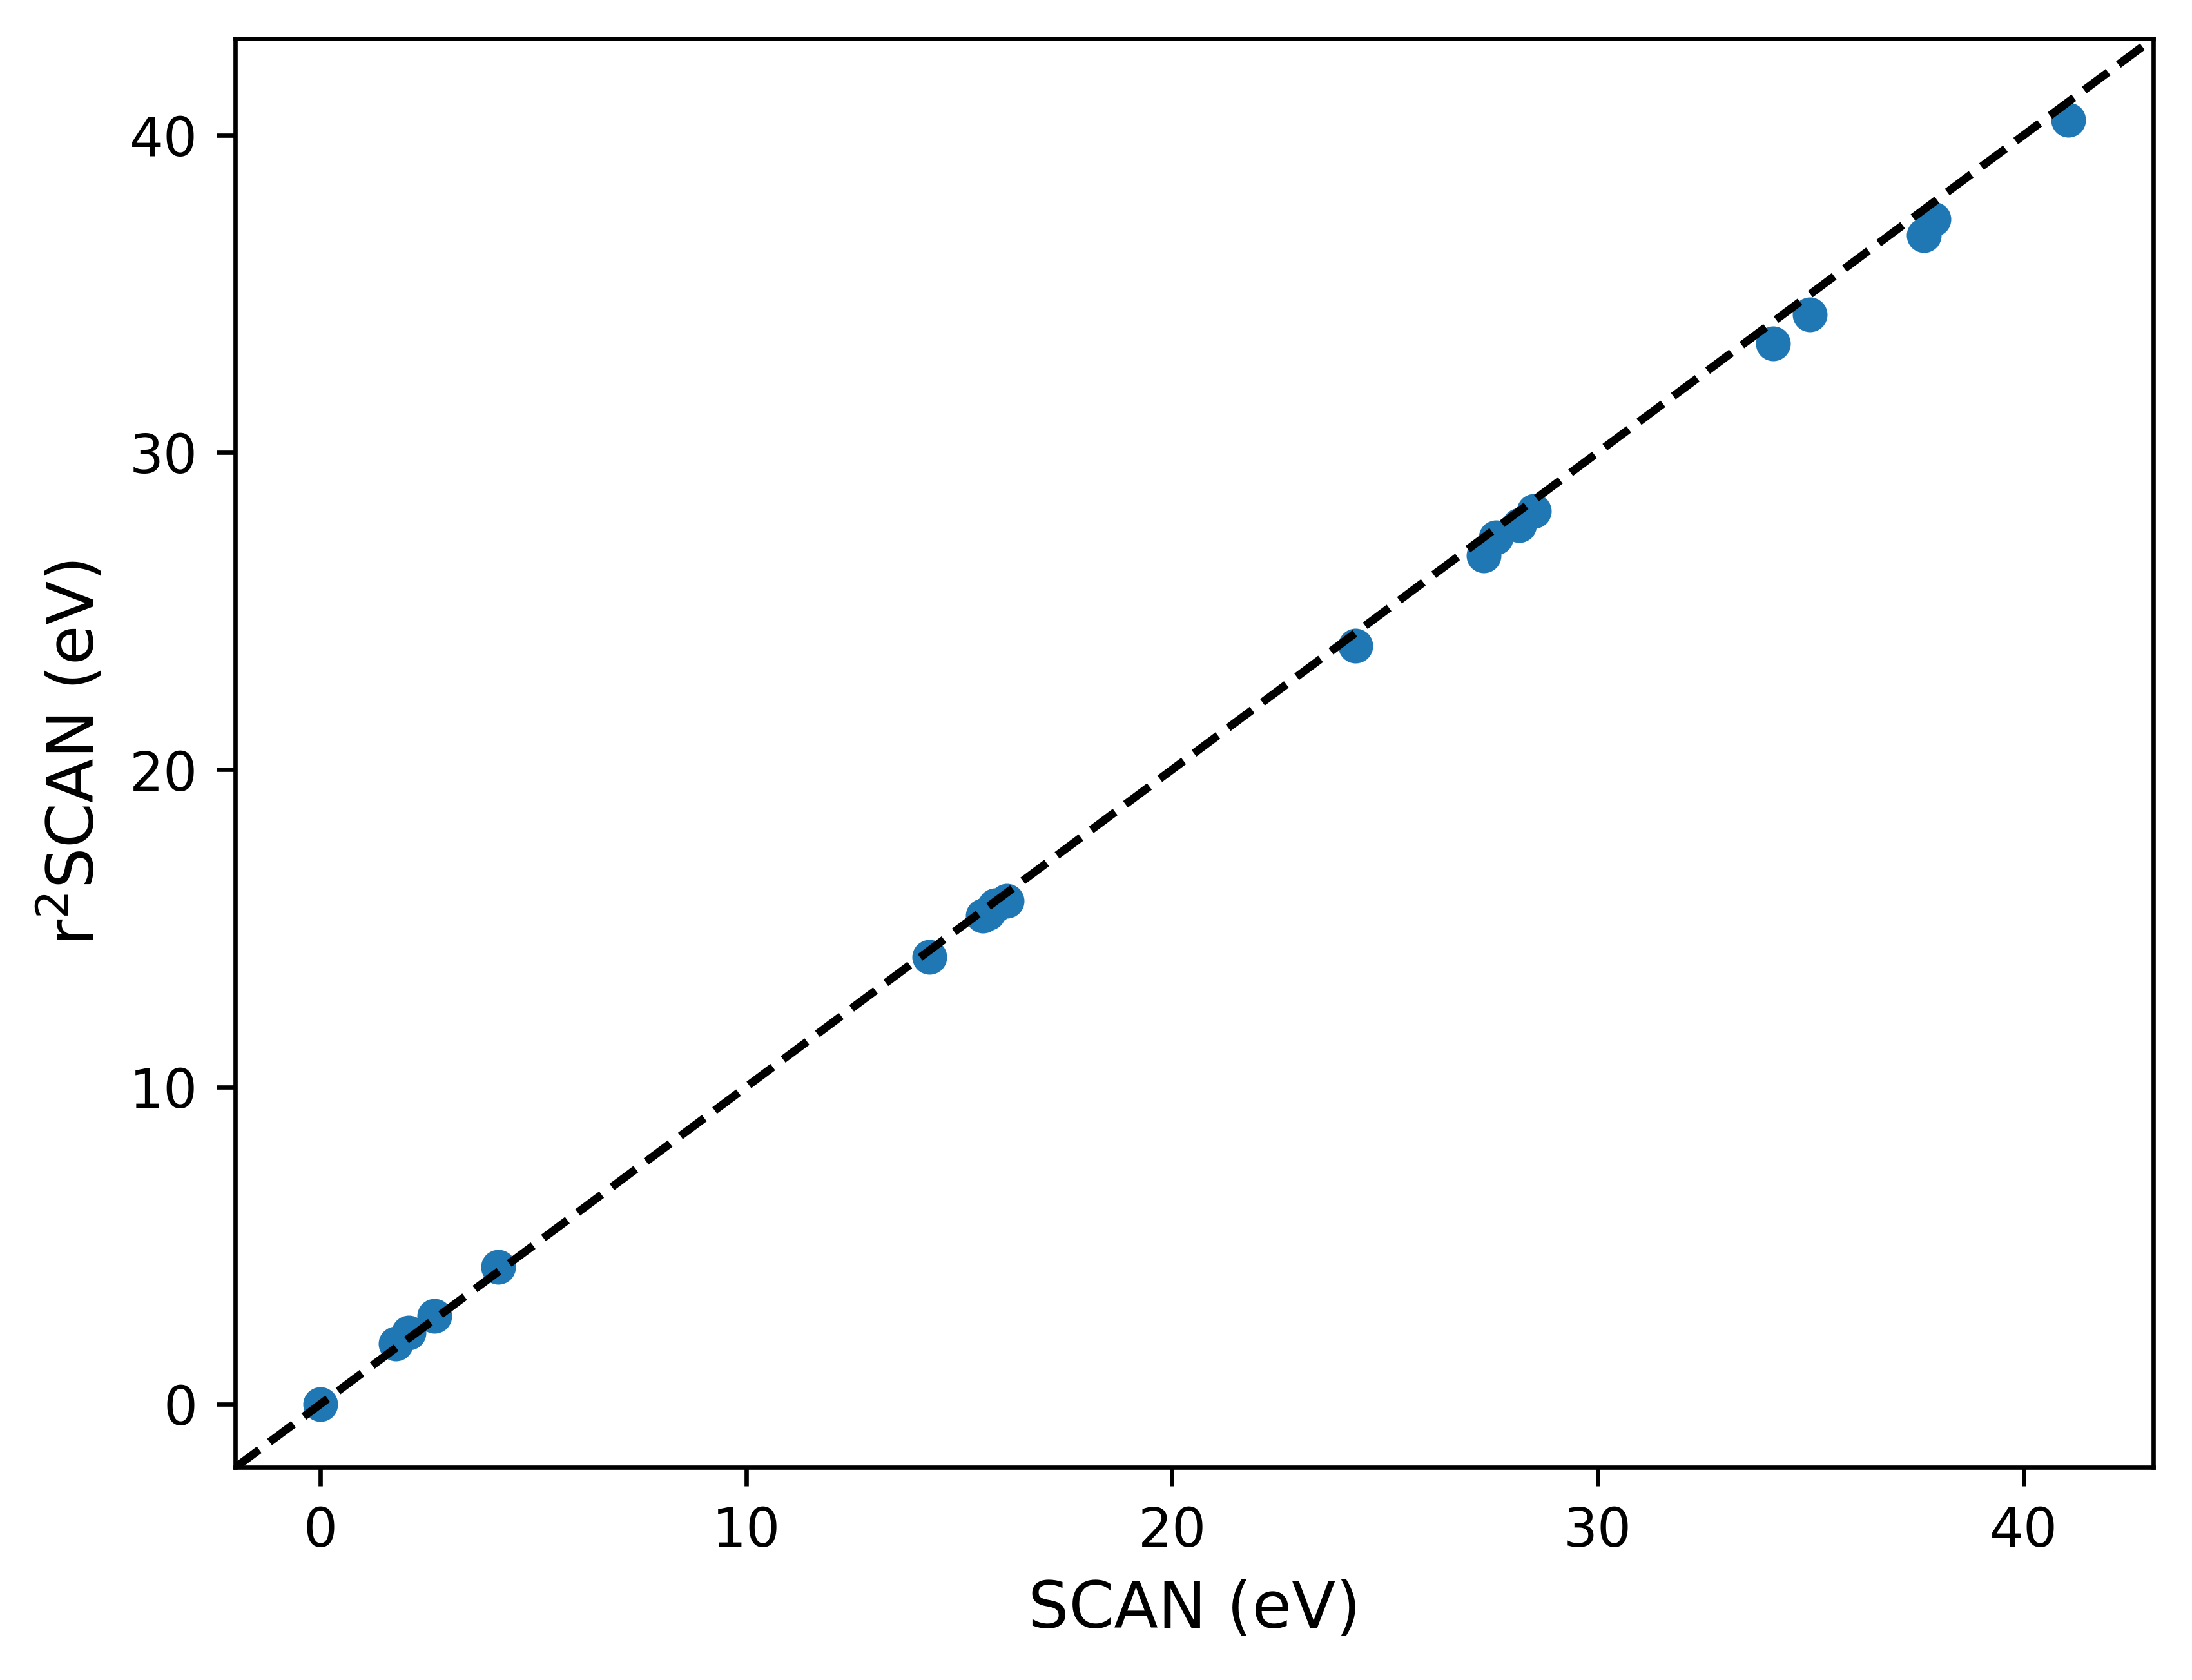
\includegraphics[width=0.9\textwidth]{images/scan_vs_r2scan/energy_compare.png}
    \caption{Energy Comparison}
    \label{fig:scan_r2scan_E}
  \end{subfigure}
  \hfill
  \begin{subfigure}{0.48\textwidth}
    \centering

    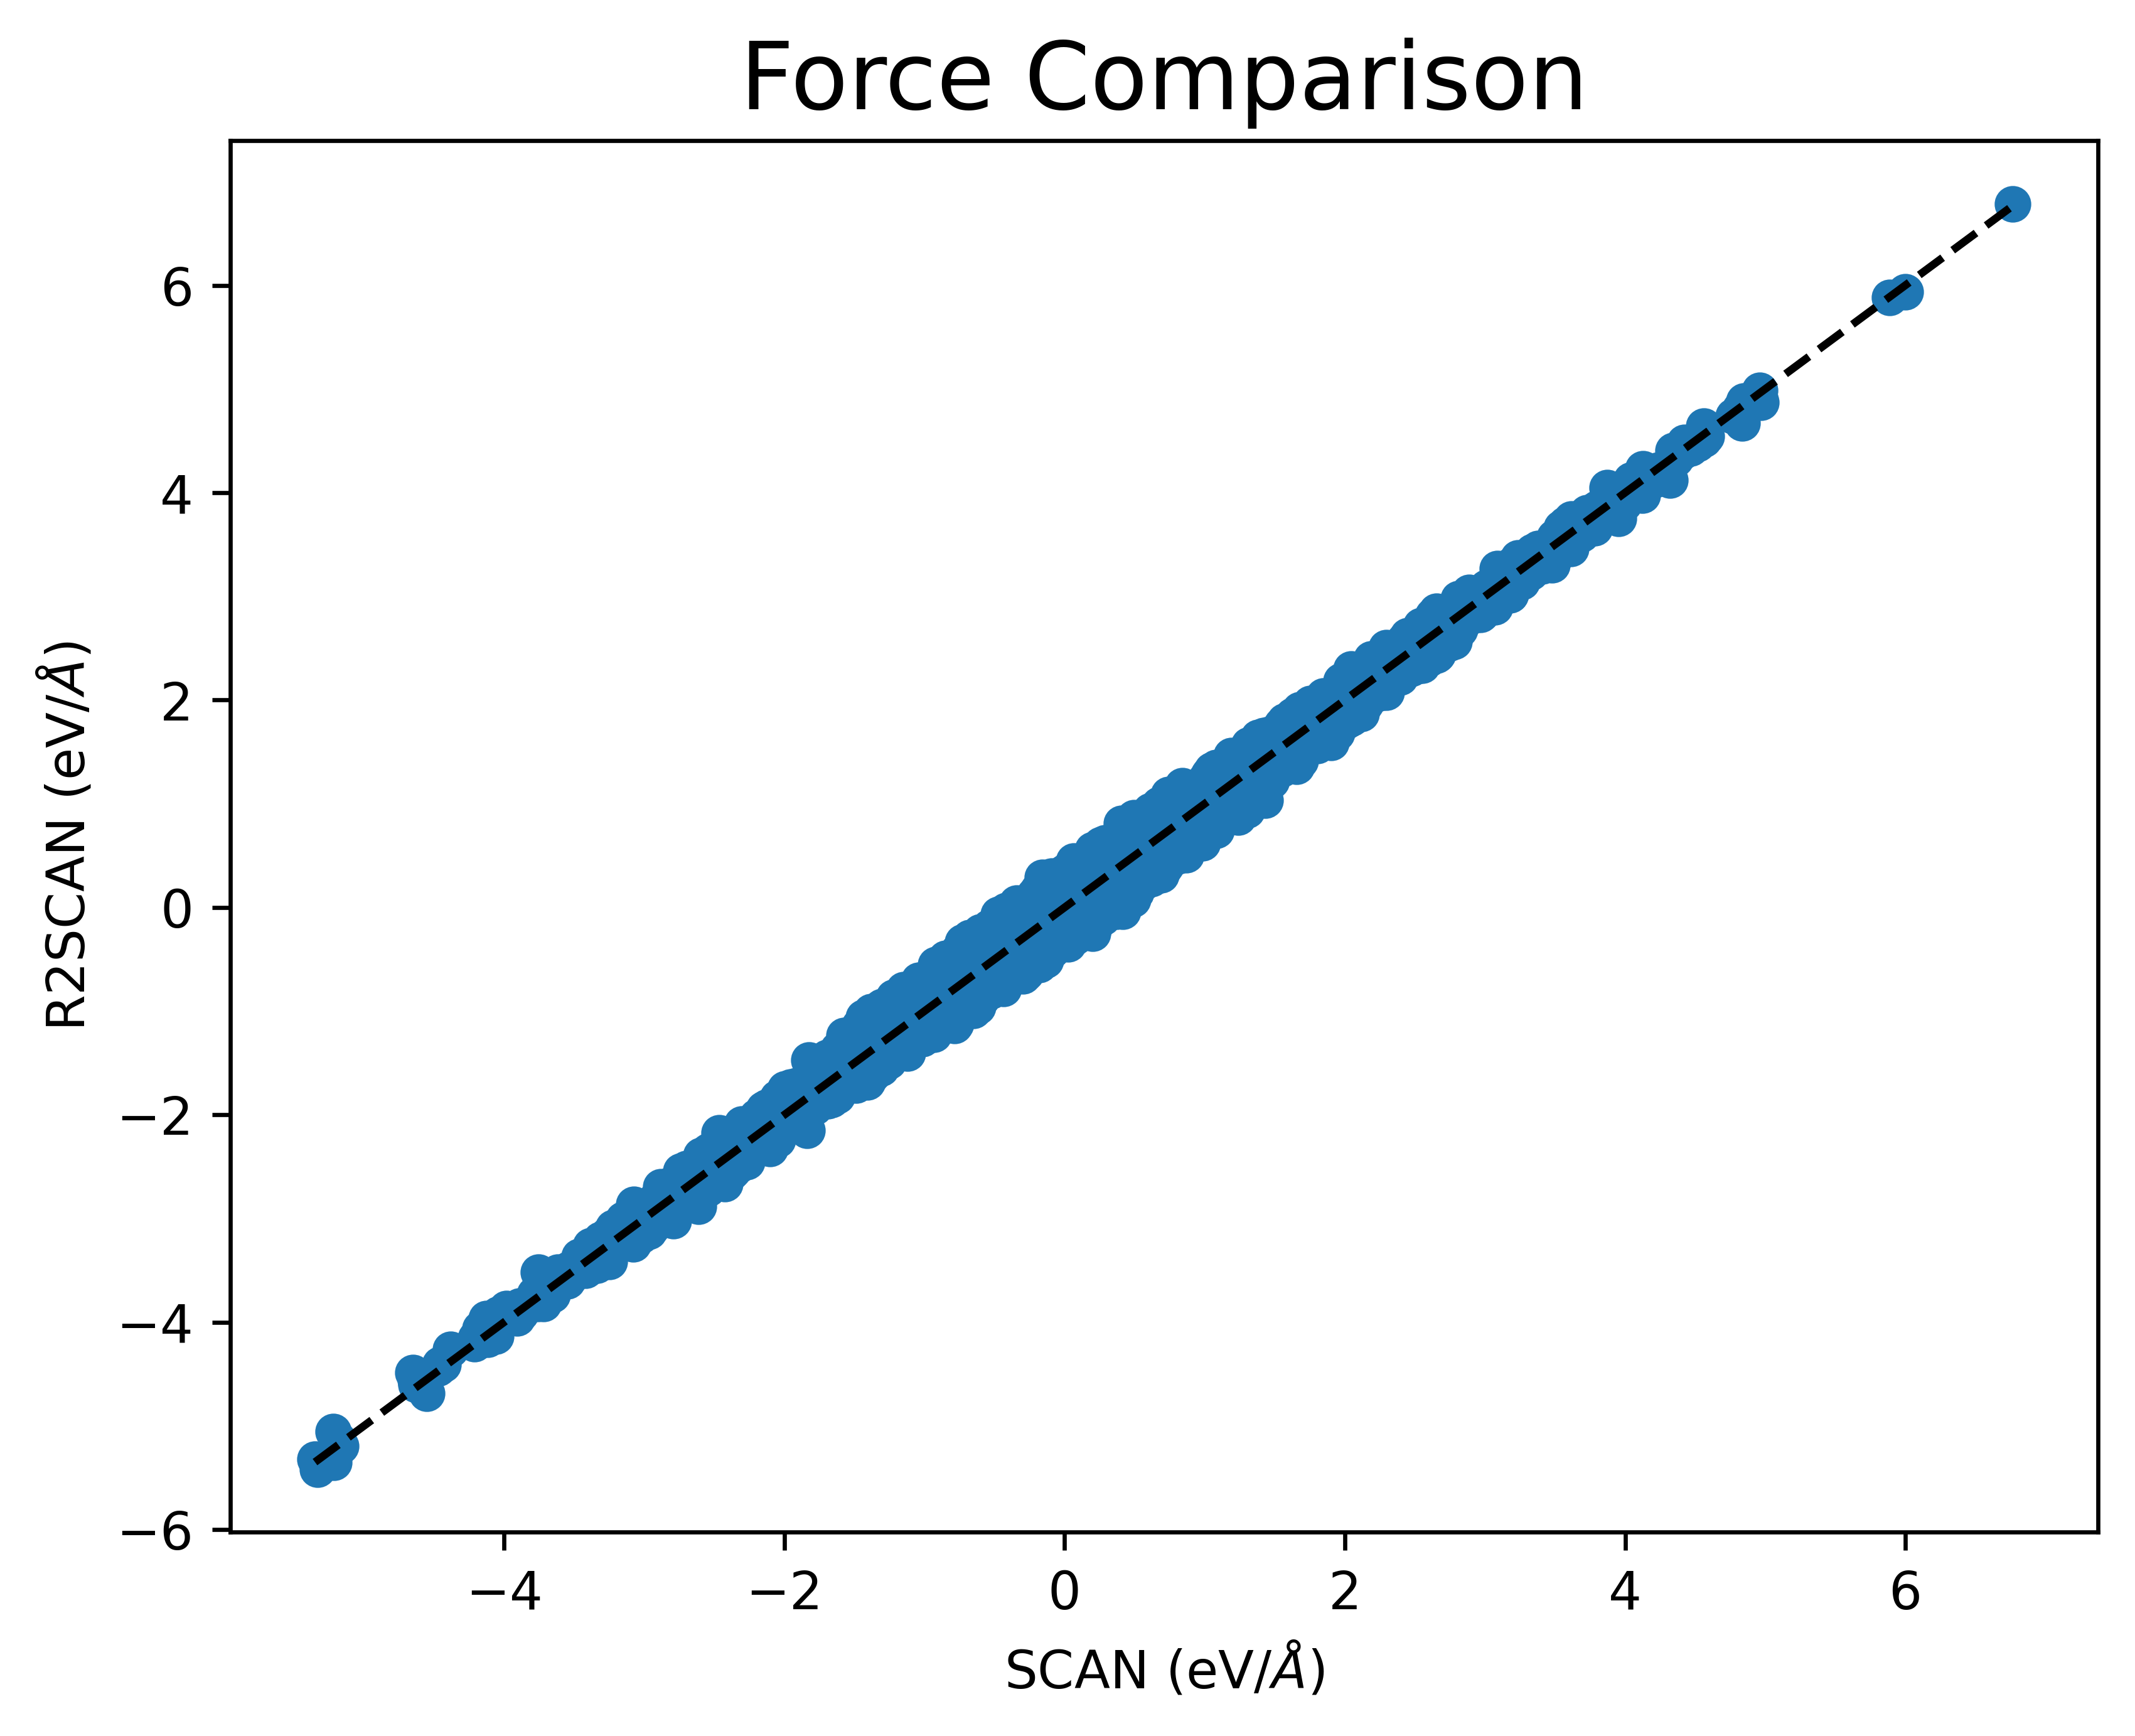
\includegraphics[width=0.9\textwidth]{images/scan_vs_r2scan/force_compare.png}
    \caption{Force Comparison}
    \label{fig:scan_r2scan_F}
  \end{subfigure}
  \hfill
  \begin{subfigure}{0.9\textwidth}
    \centering

    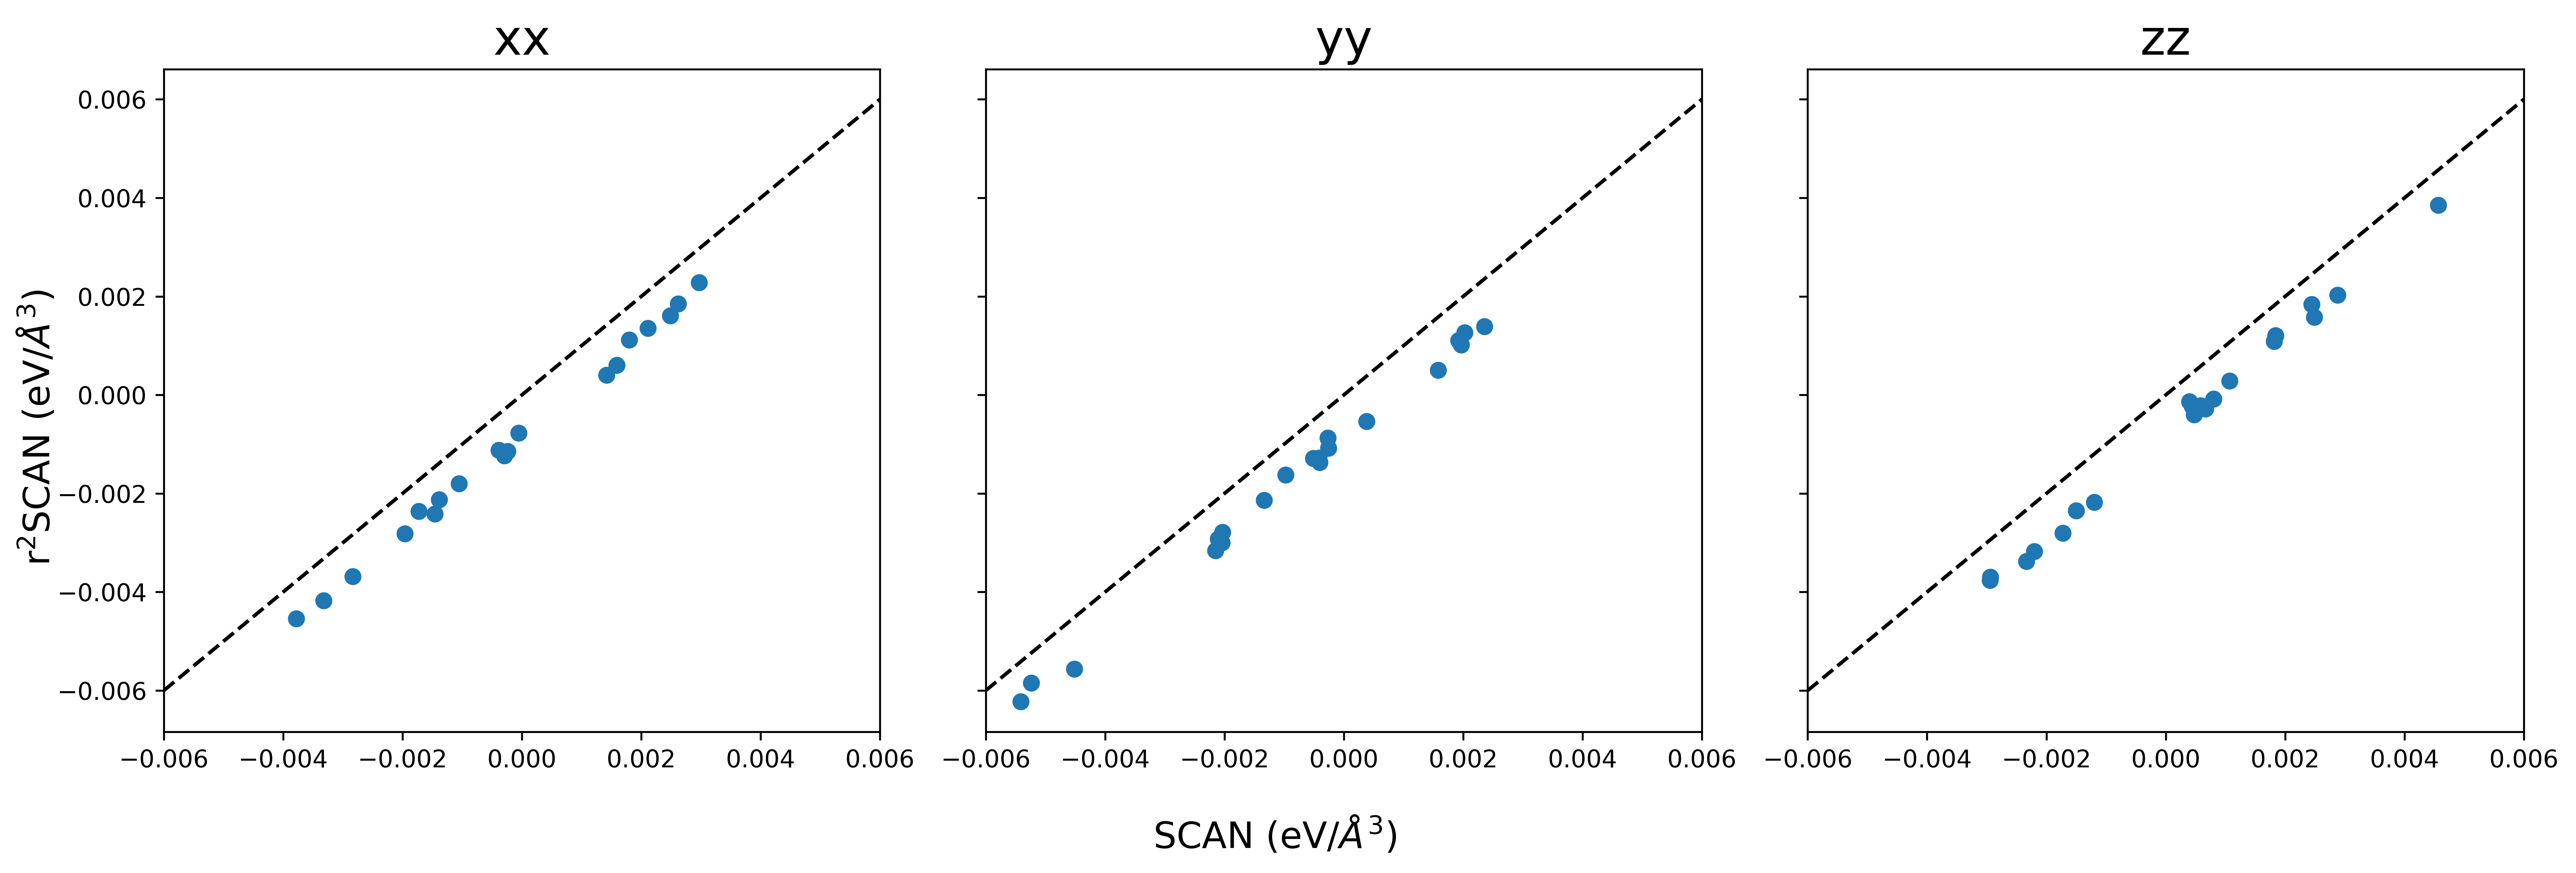
\includegraphics[width=0.9\textwidth]{images/scan_vs_r2scan/pressure_compare.png}
    \caption{Pressure Comparison}
    \label{fig:scan_r2scan_P}
  \end{subfigure}
  \caption{Correlation of  (a) energy, (b) force and (c) pressure between the
    SCAN and
    r$^2$SCAN functional. The diagonal line shows the perfect agreement between
    the two functionals.}
  \label{fig:scan_r2scan}
\end{figure}

\section{Neural Network Performance}
To check the quality of deep NN models, a test was conducted on its performance
on bulk+interface systems. Table~\ref*{tab:train_perf} lists the mean absolute
error (MAE) and root mean square error (RMSE) of bulk trained NNP and
bulk+interface trained NNP for system's properties such as energy, force, and
virial stress. It can be observed that the error is lower when the NNP is
trained to include both bulk  and interfaces. This is expected since the model
was trained to explore both the bulk and interface environments.
\begin{table}[tbhp!]
  \centering
  \caption{Performance of bulk trained NNP and
    bulk+interface trained NNP on bulk+interface validation dataset.}
  \label{tab:train_perf}
  \resizebox{0.7\columnwidth}{!}{%
    \begin{tabular}{@{}lcc@{}}
      \toprule
                                & Bulk trained NNP & Bulk+Interface trained NNP
      \\
      \midrule
      Energy MAE (eV)           & \num{5.195E-01}  & \num{1.939E-01}
      \\
      Energy   RMSE   (eV)      & \num{6.222E-01}  & \num{2.616E-01}
      \\
      Energy MAE/Natoms (eV)    & \num{9.019E-04}  & \num{3.366E-04}
      \\
      Energy   RMSE/Natoms (eV) & \num{1.080E-03}  & \num{4.541E-04}
      \\
      Force  MAE	(eV/A)          & \num{4.164E-02}  & \num{3.613E-02}
      \\
      Force  RMSE (eV/A)        & \num{5.654E-02}  & \num{4.836E-02}
      \\
      Virial MAE (eV)           & \num{5.886E-01}  & \num{5.491E-01}
      \\
      Virial   RMSE (eV)        & \num{7.924E-01}  & \num{7.256E-01}
      \\
      Virial MAE/Natoms (eV)    & \num{1.020E-03}  & \num{9.533E-04}
      \\
      Virial   RMSE/Natoms (eV) & \num{1.380E-03}  & \num{1.260E-03}
      \\
      \bottomrule
    \end{tabular}%
  }
\end{table}

We check the correlation between the deep NN prediction with the DFT data.
Figure~\ref{fig:corr_bulk_NN} shows points whose coordinates are the DFT data
and the predicted ones given
by the neural network for a bulk-only trained potential. In particular, it can
be seen that the predicted energies are mostly underestimated which leads to
higher test error as supported in Table~\ref{tab:train_perf}. The forces are in
good agreement. However, the predicted $zz$ components of virial tensor are
mostly overestimated. In contrast, Figure~\ref{fig:corr_bulk+interface_NN}
shows good agreement across all parameters for a neural network potential
trained on bulk and interface environments.

\begin{figure}[tbhp]
  \centering
  \begin{subfigure}{0.48\textwidth}
    \centering

    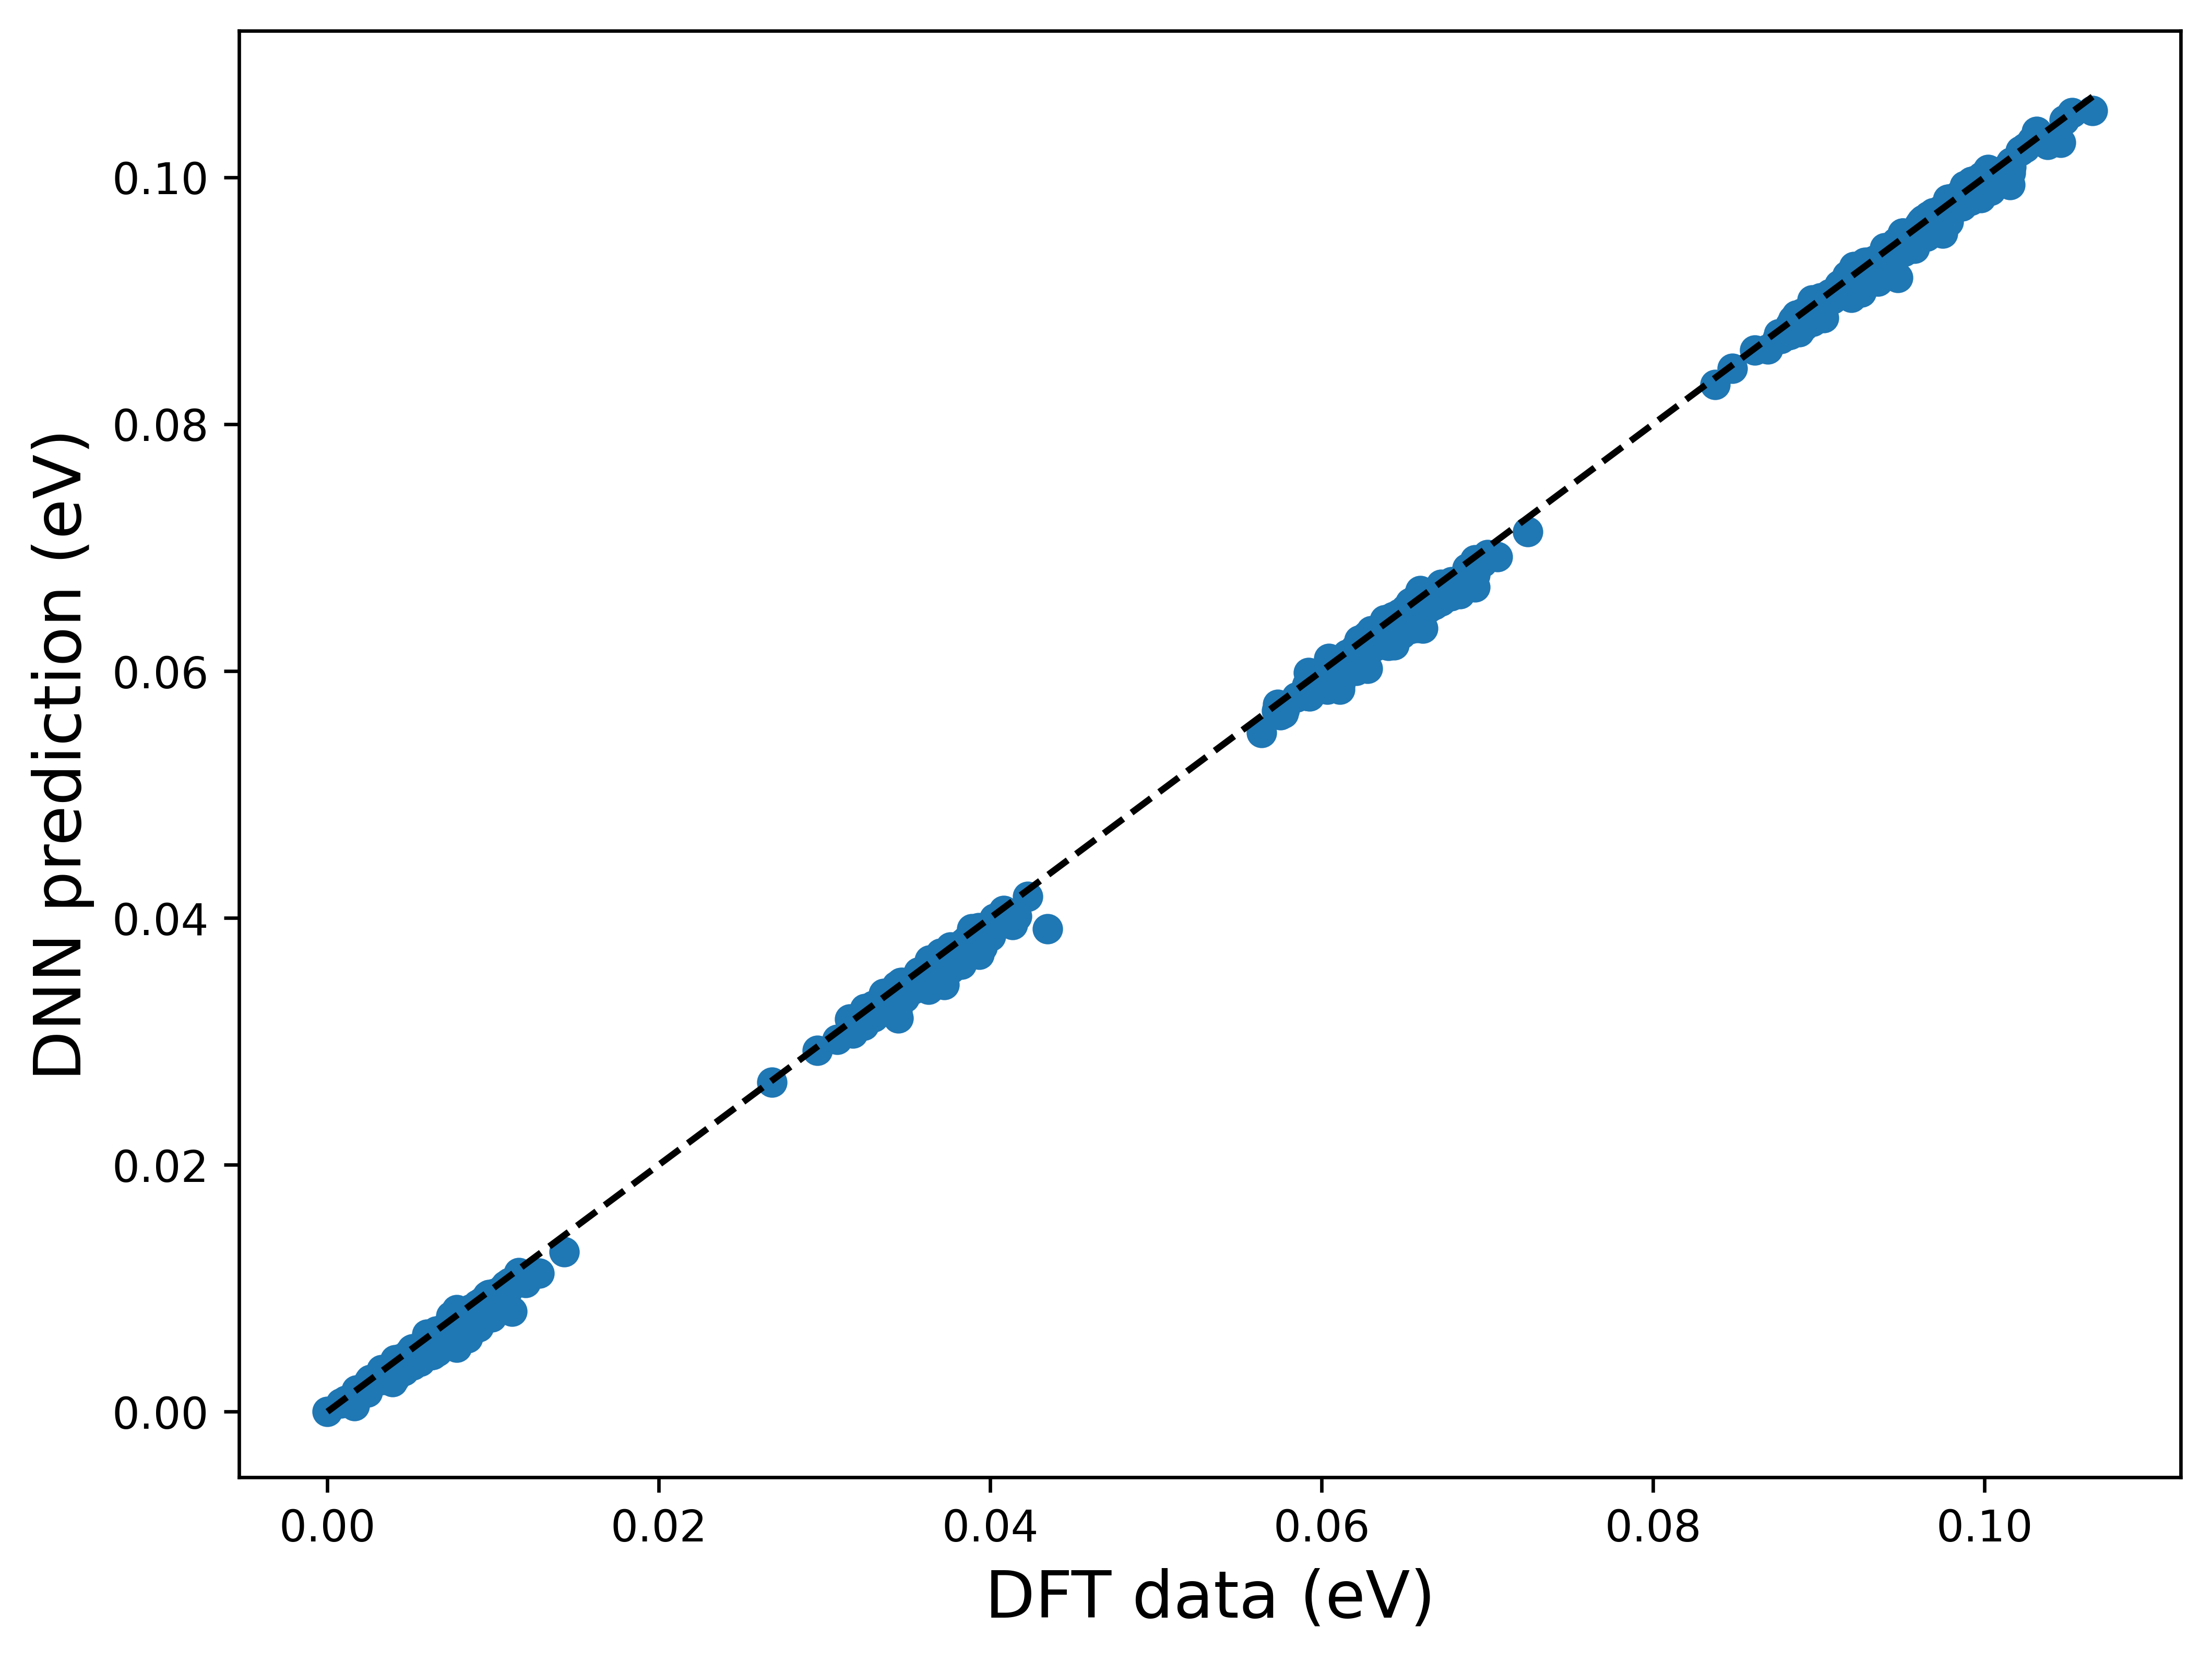
\includegraphics[width=0.9\textwidth]{images/bulk_NN_on_interface/2_e_peratom.png}
    \caption{Energy per atom}
    \label{fig:corr_bulk_NN_E}
  \end{subfigure}
  \hfill
  \begin{subfigure}{0.48\textwidth}
    \centering

    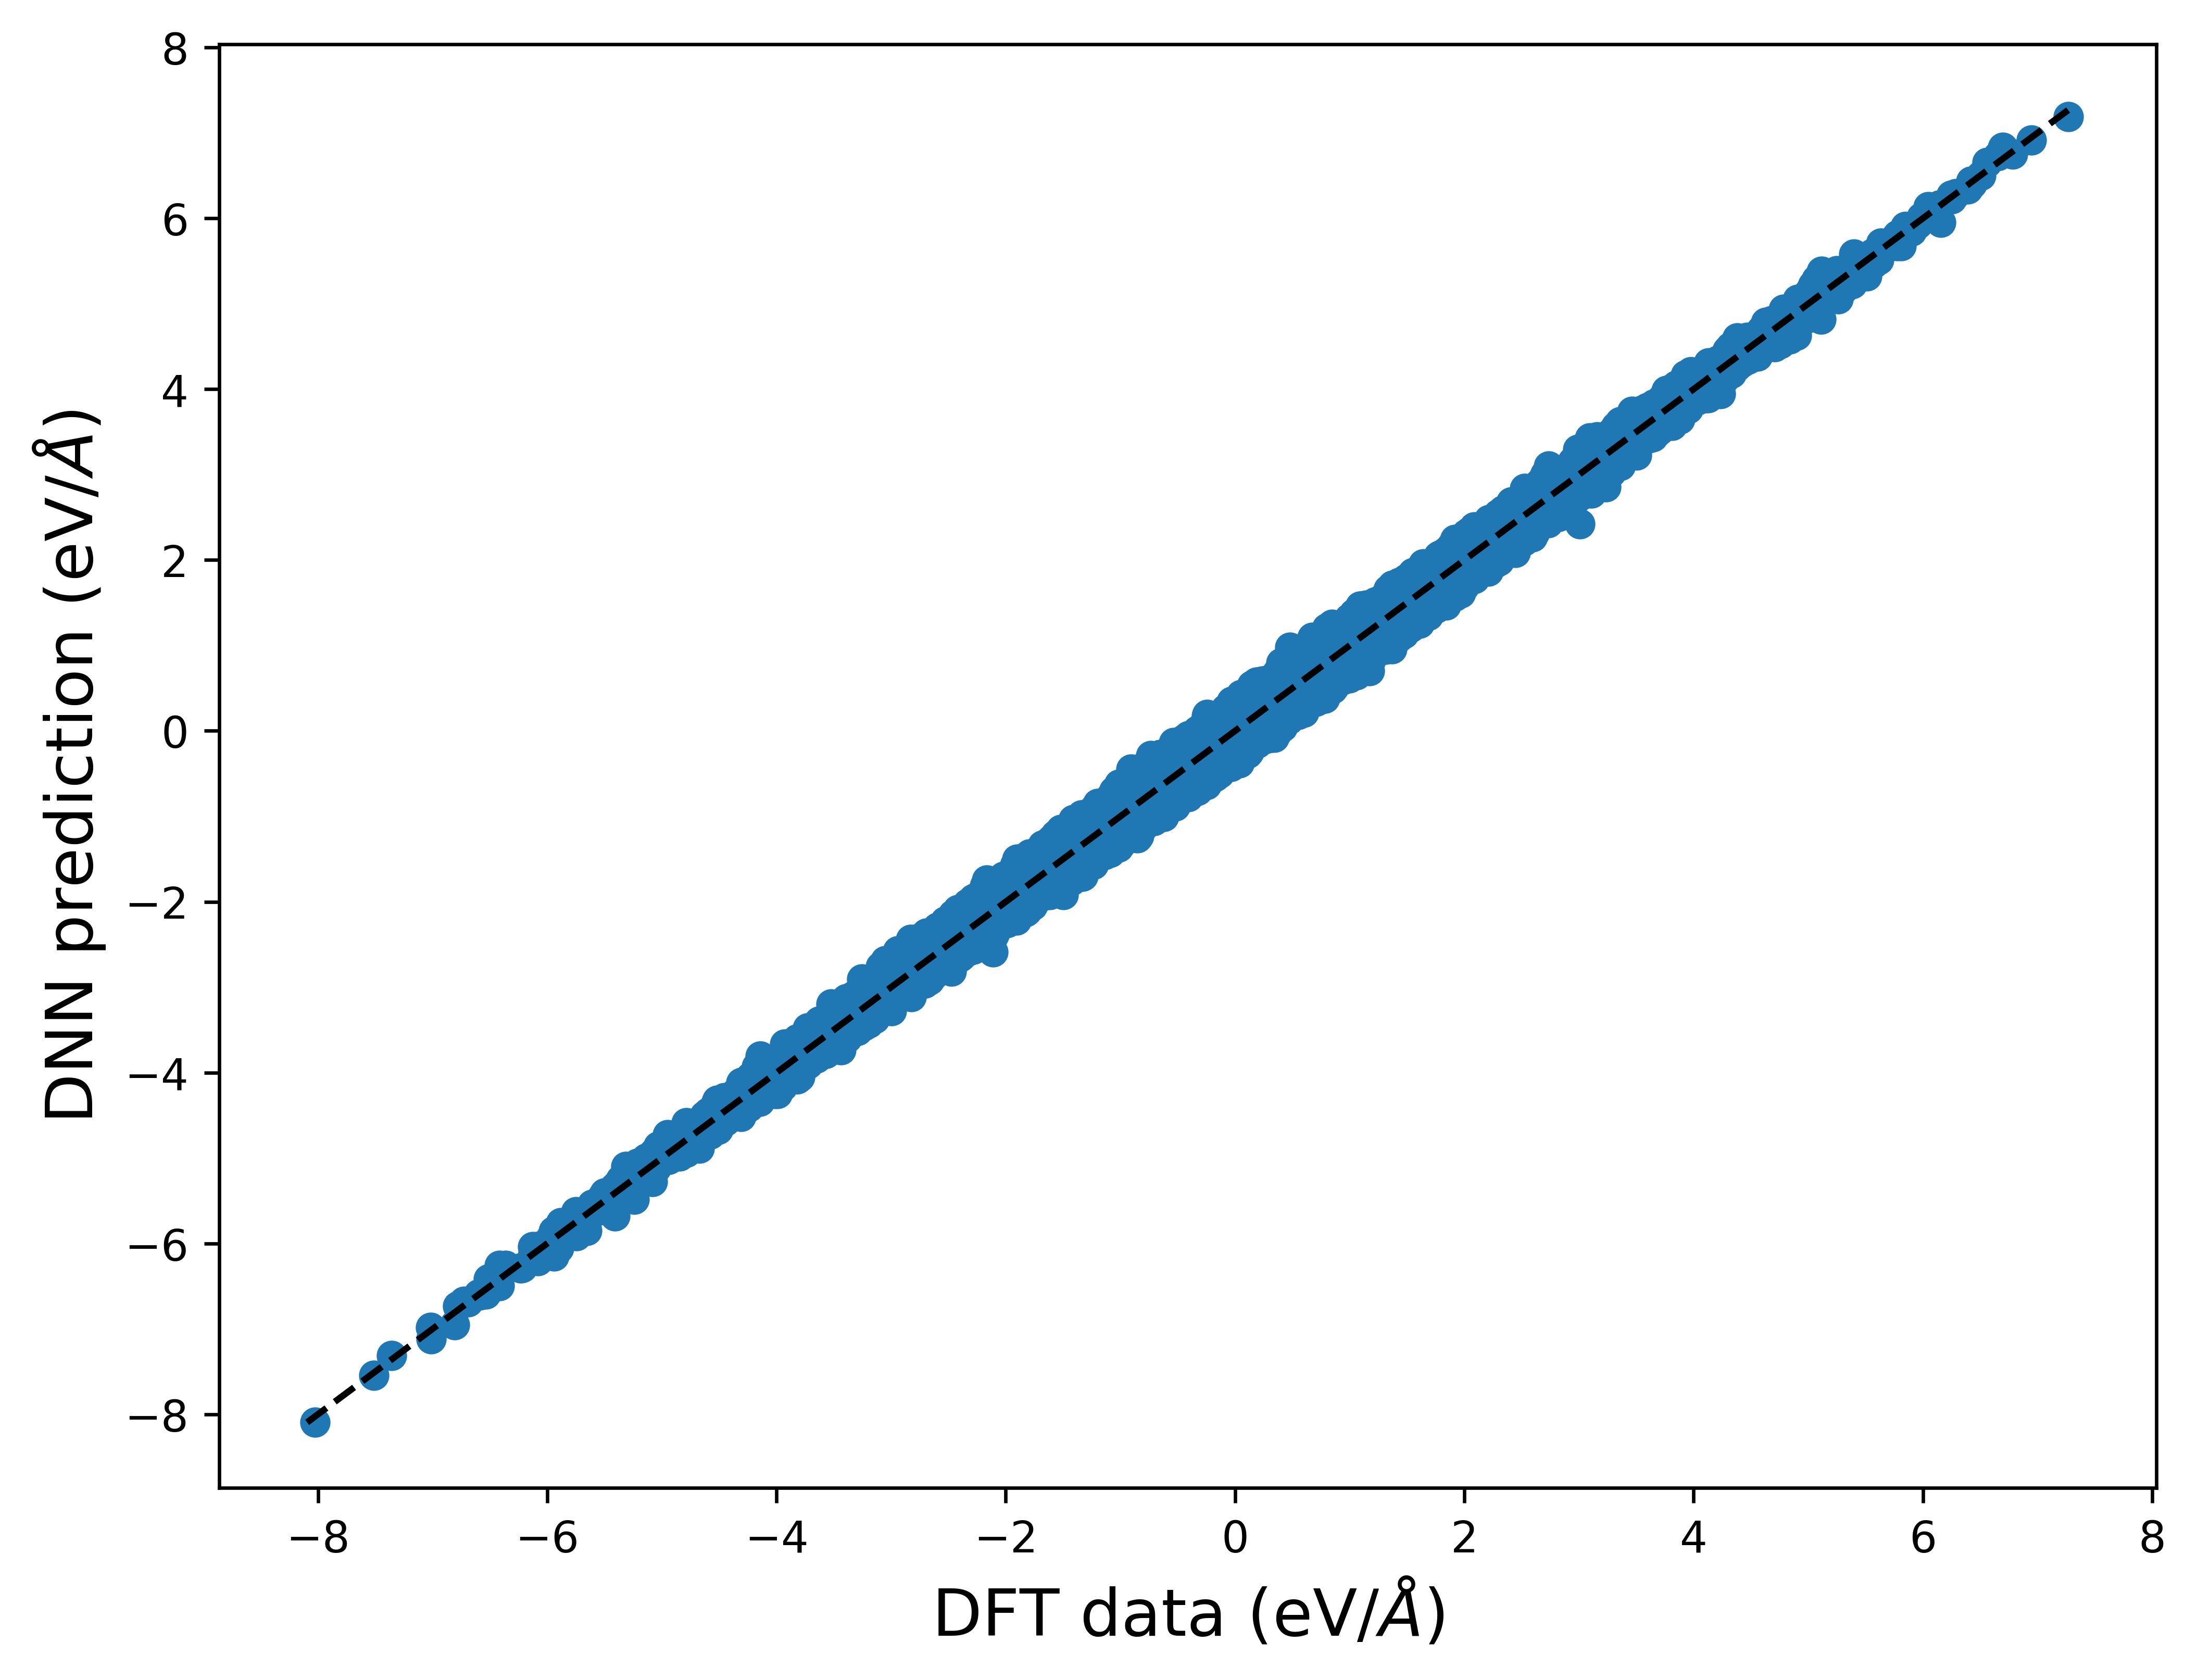
\includegraphics[width=0.9\textwidth]{images/bulk_NN_on_interface/2_force.png}
    \caption{Force }
    \label{fig:corr_bulk_NN_F}
  \end{subfigure}
  \hfill
  \begin{subfigure}{0.9\textwidth}
    \centering

    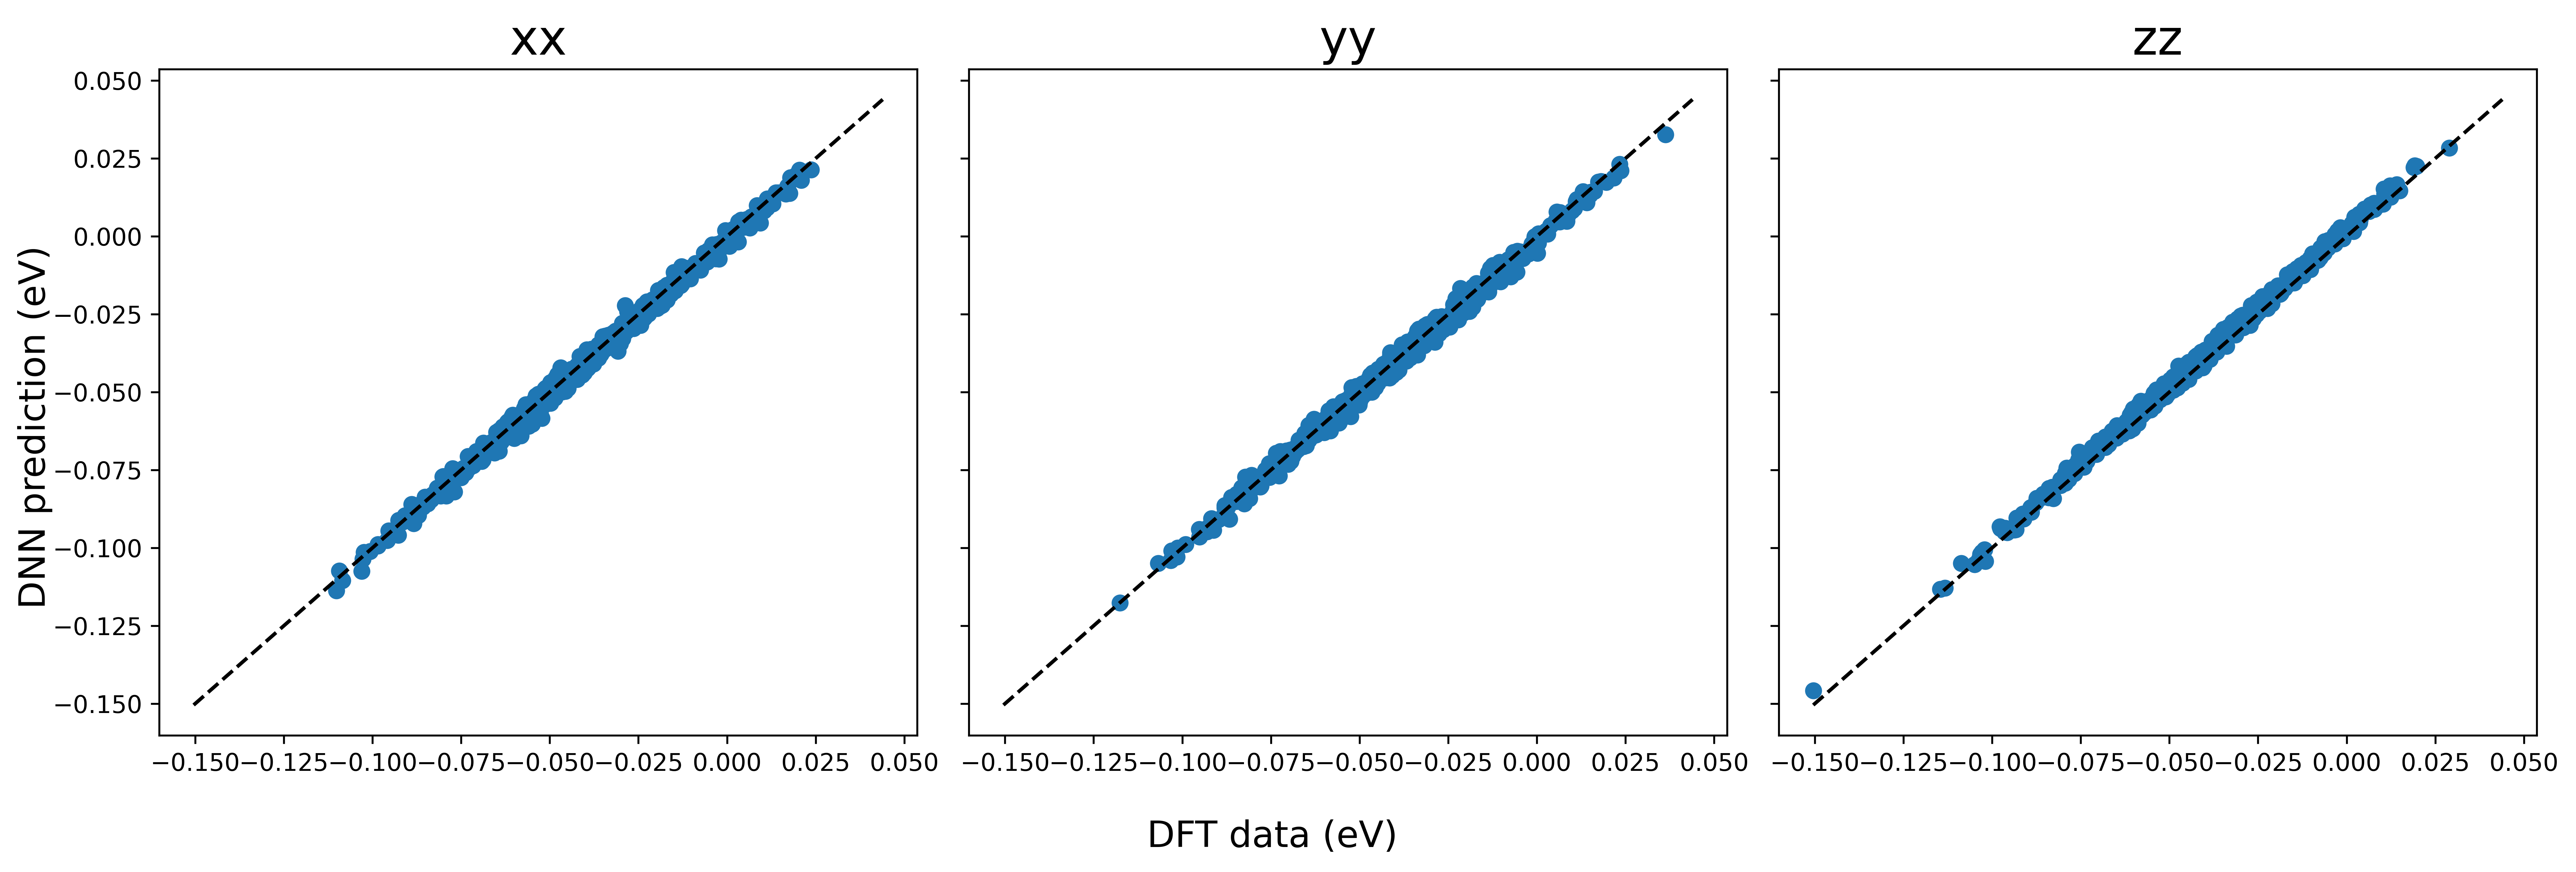
\includegraphics[width=0.9\textwidth]{images/bulk_NN_on_interface/2_virial_peratom.png}
    \caption{Virial per atom}
    \label{fig:corr_bulk_NN_P}
  \end{subfigure}
  \caption{Correlation between deep NN prediction data with the DFT data for a
    model trained on bulk system. The
    diagonal line shows the perfect agreement between the two data.}
  \label{fig:corr_bulk_NN}
\end{figure}

\begin{figure}[tbhp]
  \centering
  \begin{subfigure}{0.48\textwidth}
    \centering

    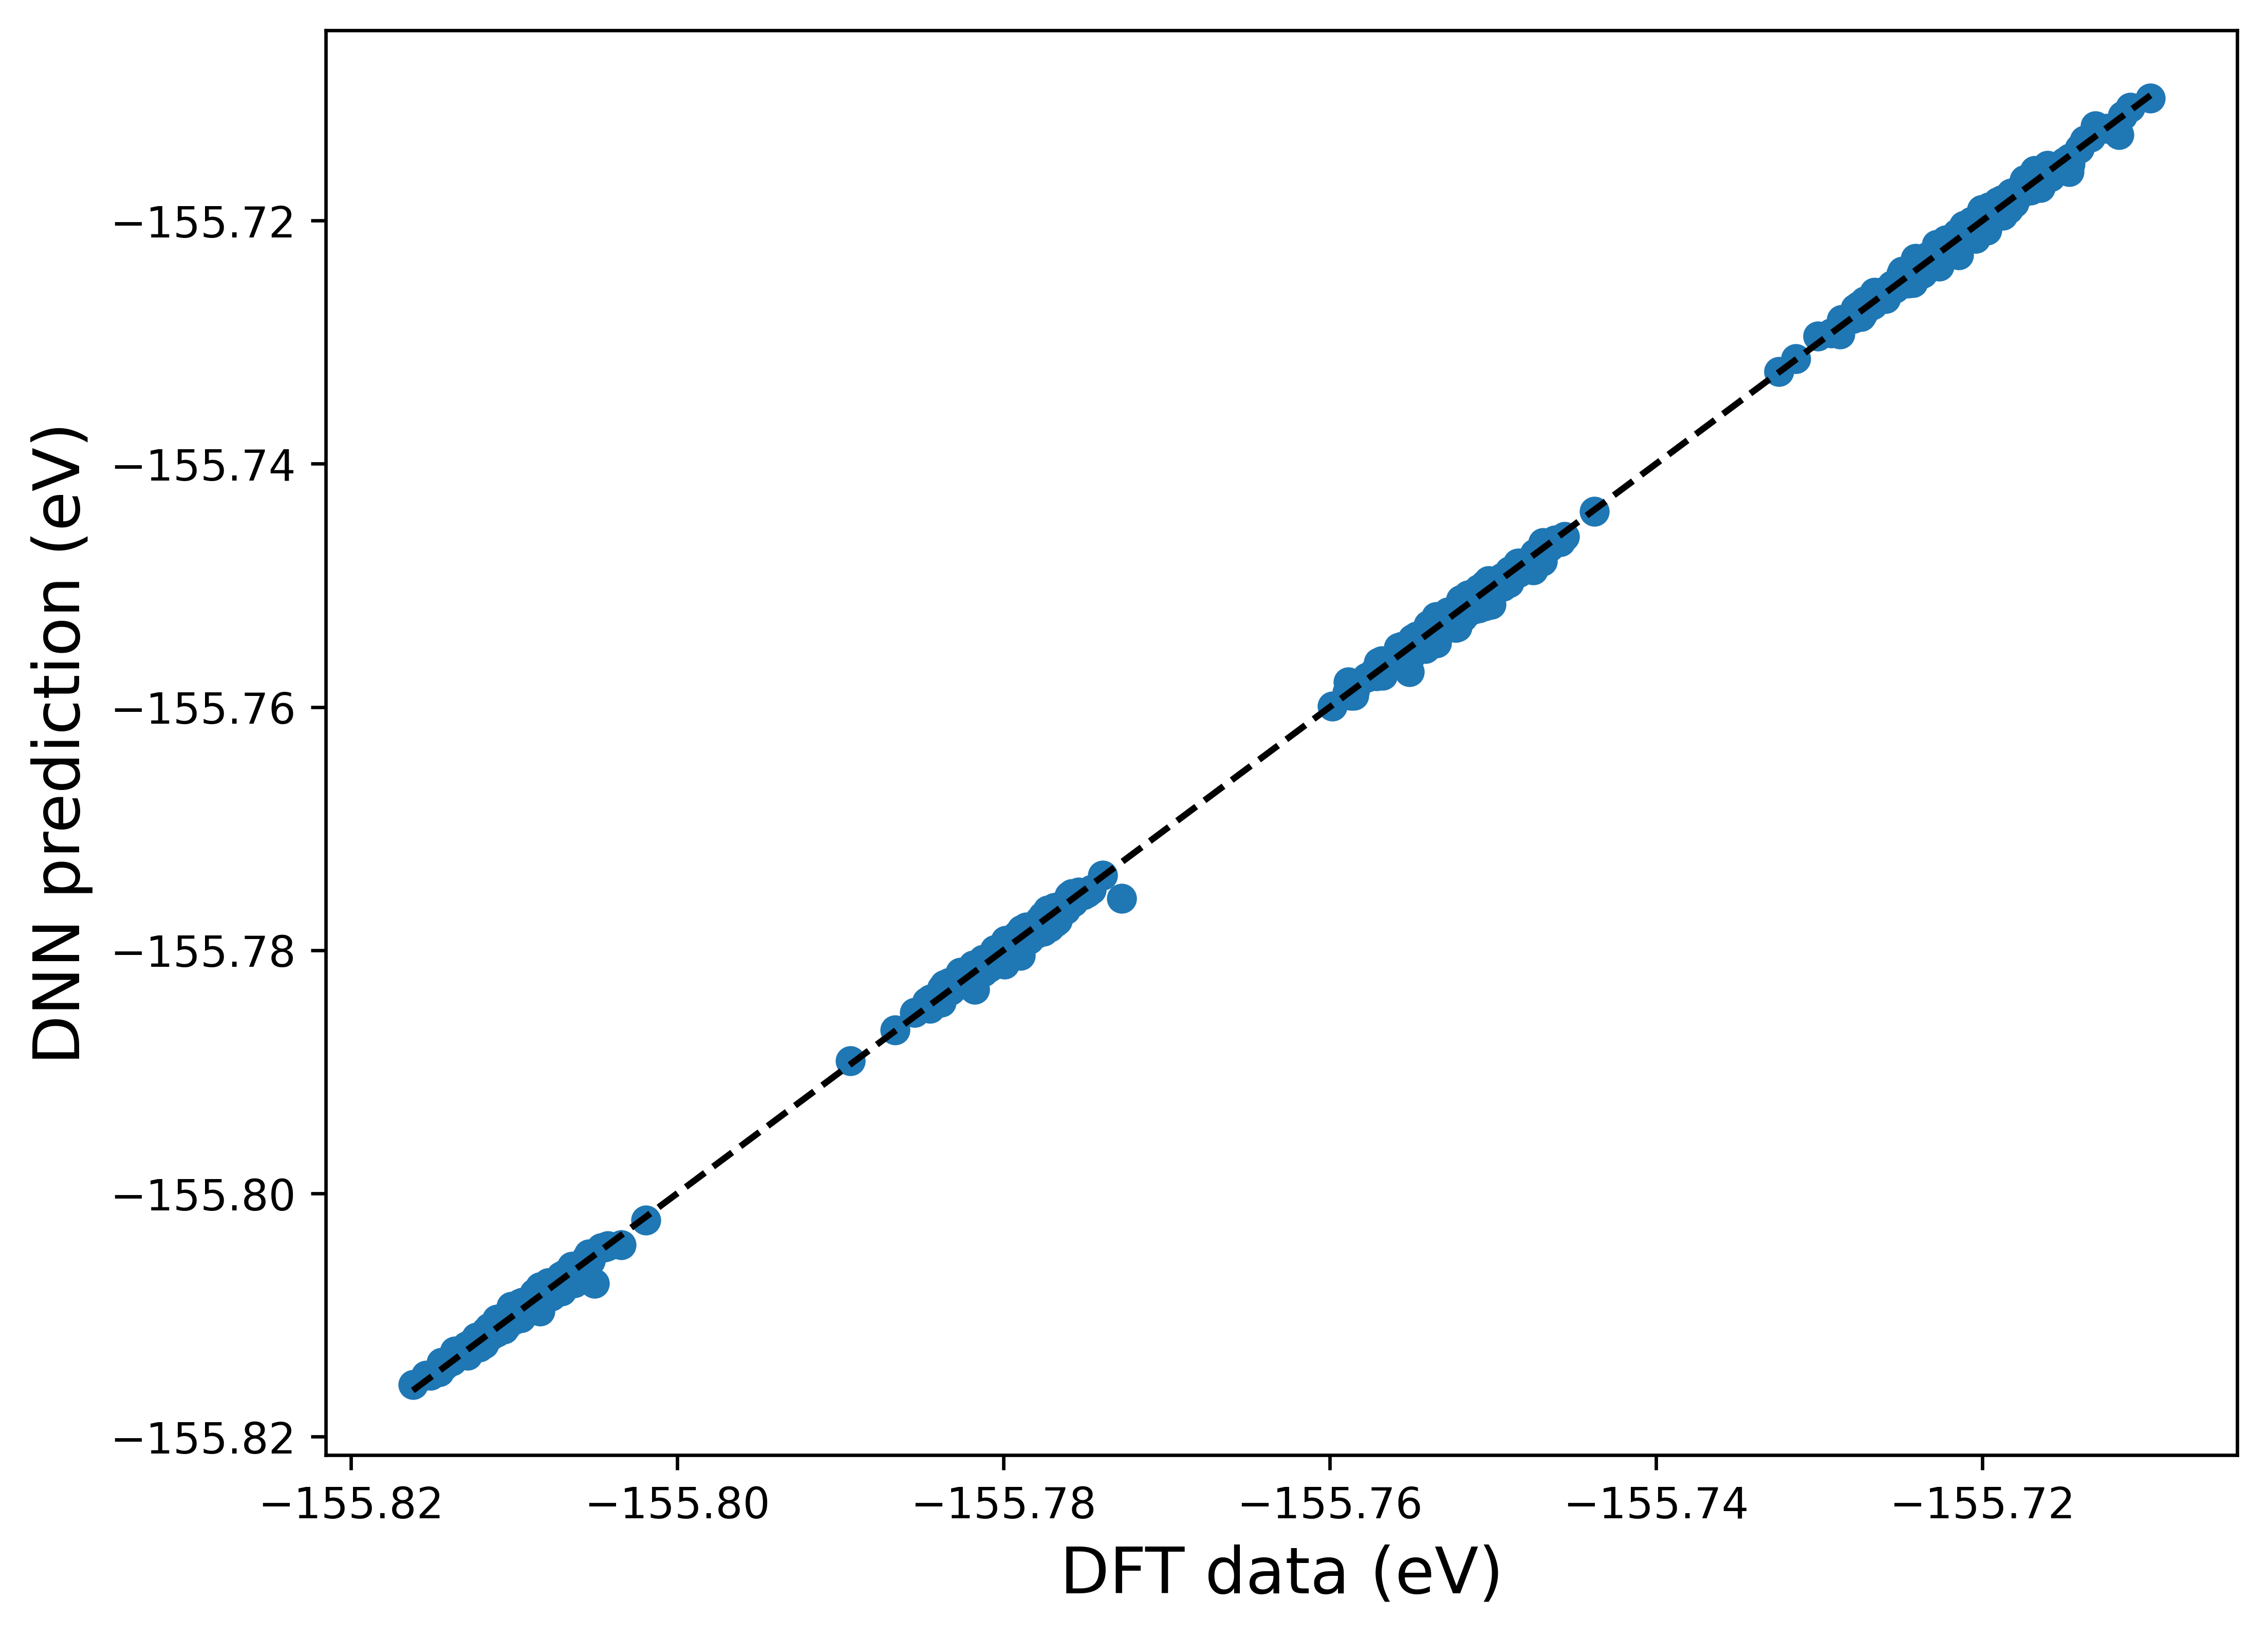
\includegraphics[width=0.9\textwidth]{images/bulk+interface_NN_on_interface/2_e_peratom.png}
    \caption{Energy per atom}
    \label{fig:corr_bulk+interface_NN_E}
  \end{subfigure}
  \hfill
  \begin{subfigure}{0.48\textwidth}
    \centering

    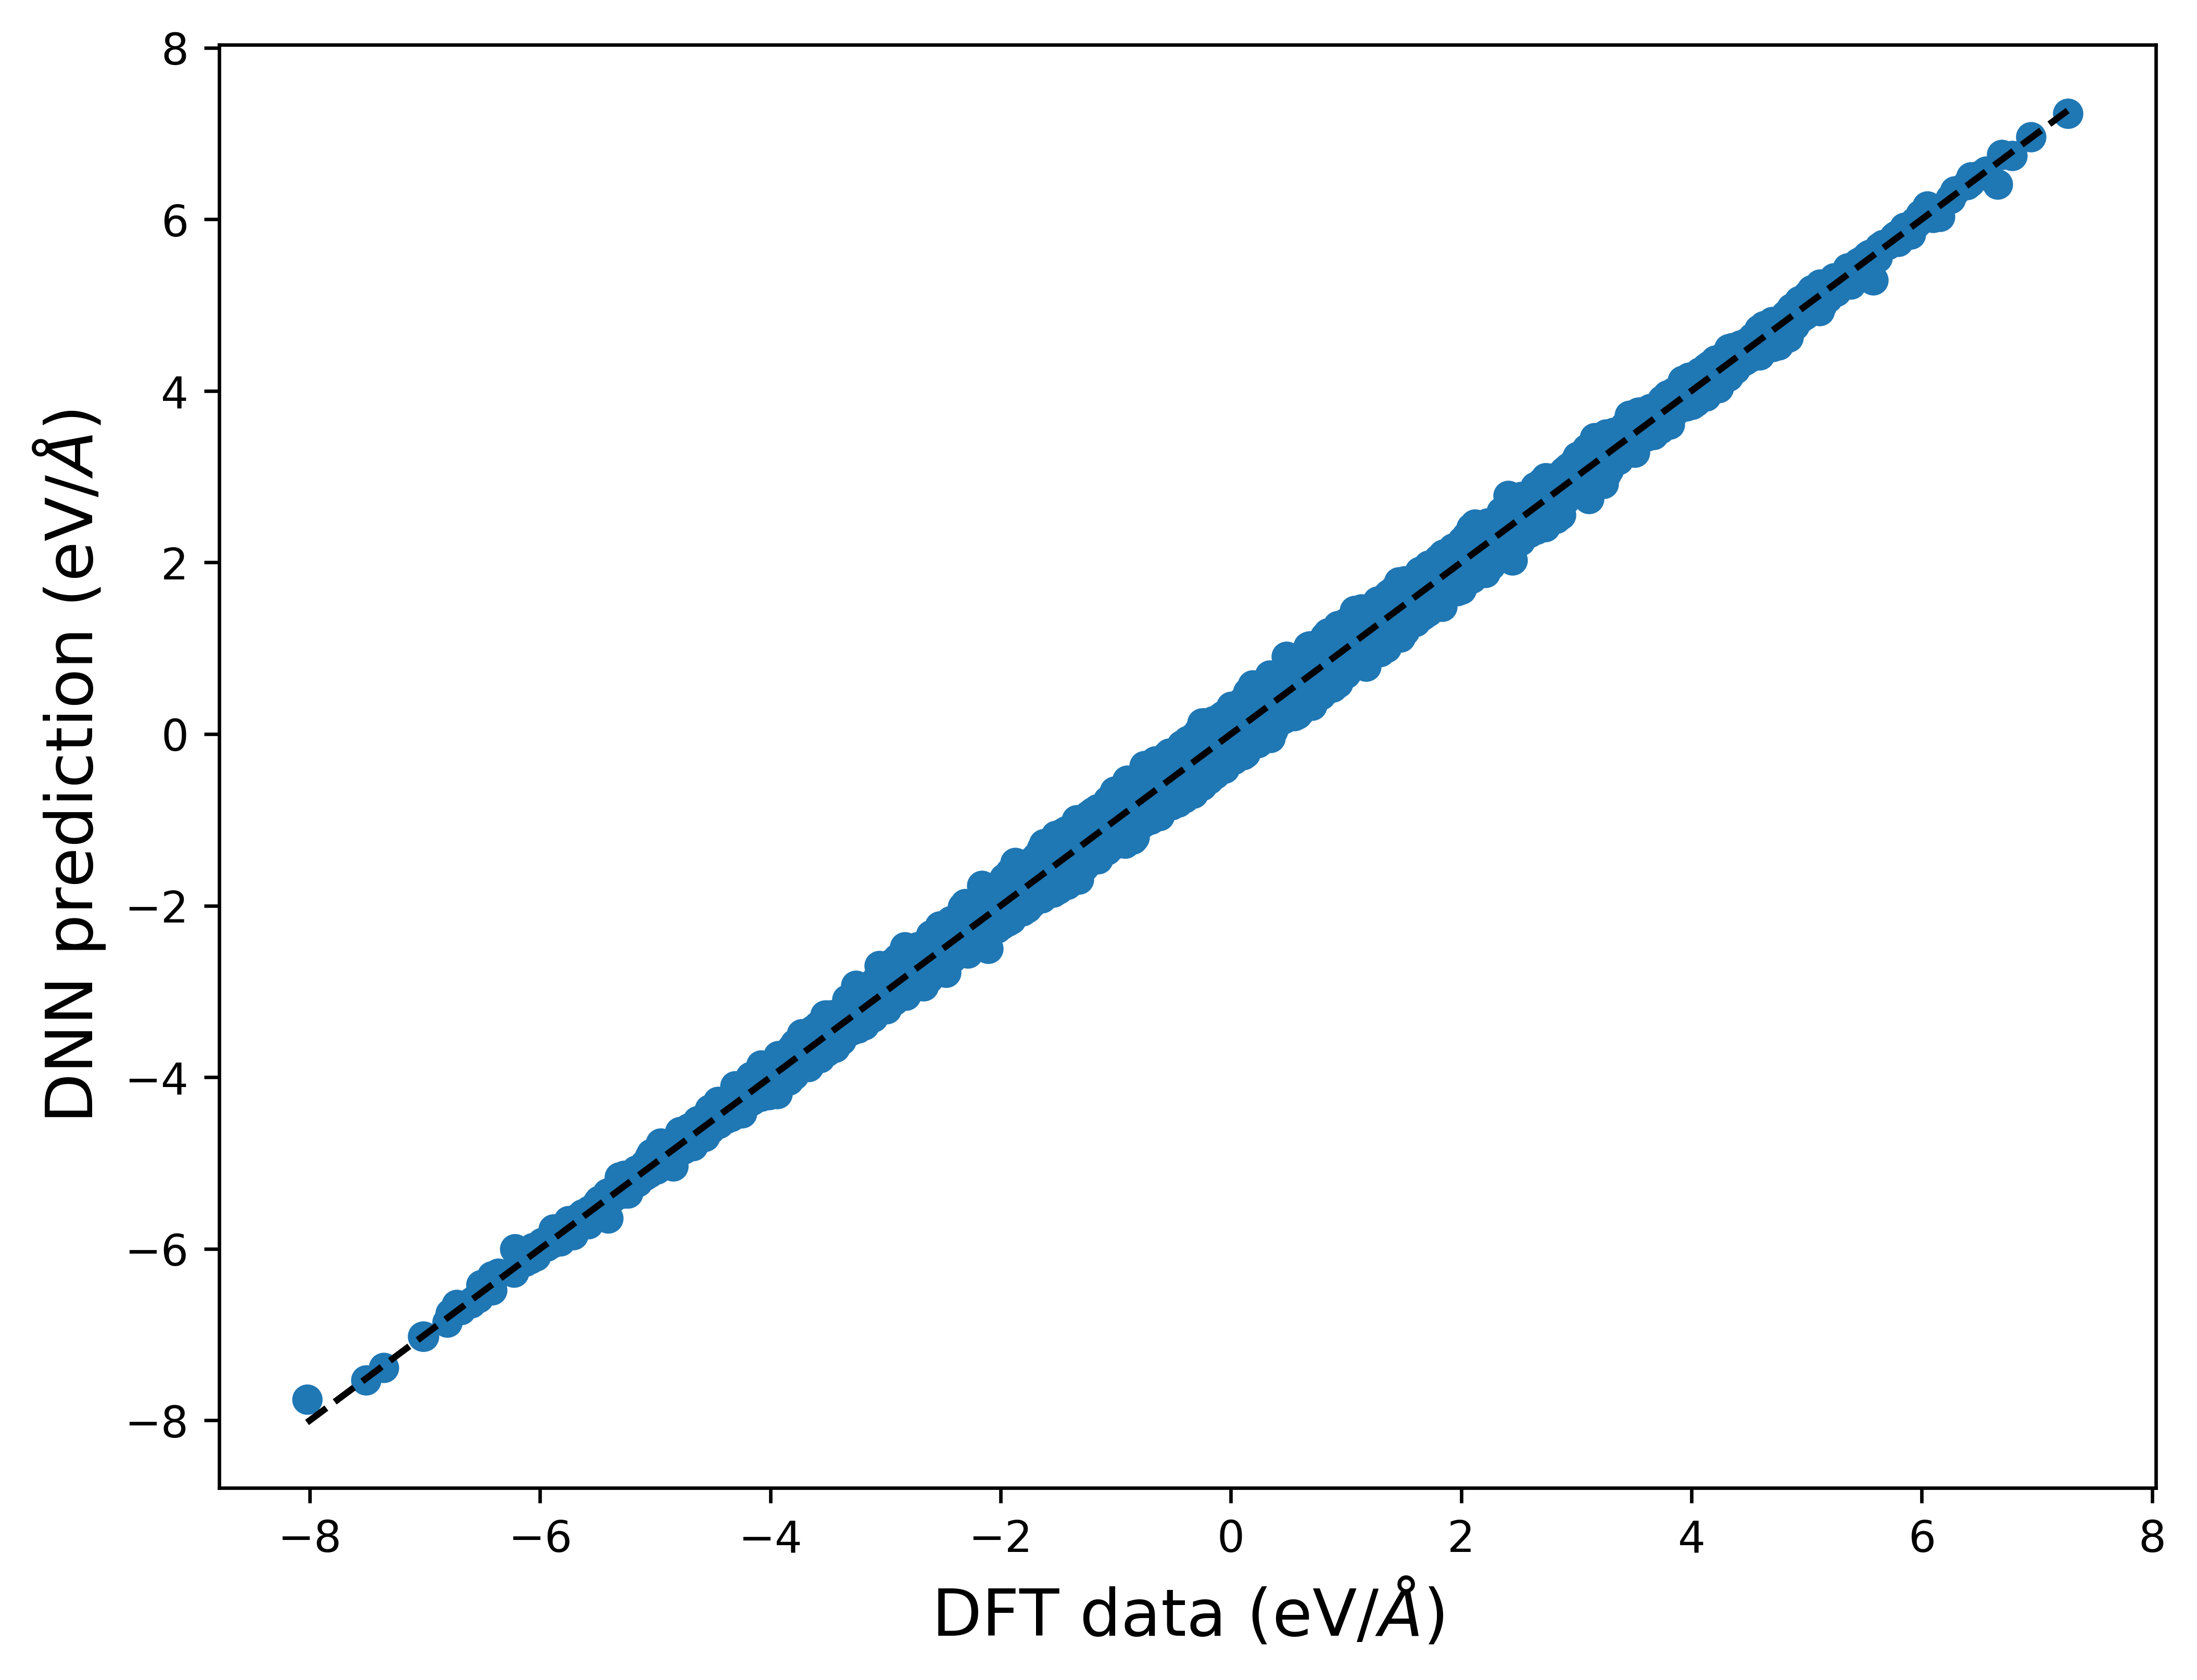
\includegraphics[width=0.9\textwidth]{images/bulk+interface_NN_on_interface/2_force.png}
    \caption{Force }
    \label{fig:corr_bulk+interface_NN_F}
  \end{subfigure}
  \hfill
  \begin{subfigure}{0.9\textwidth}
    \centering

    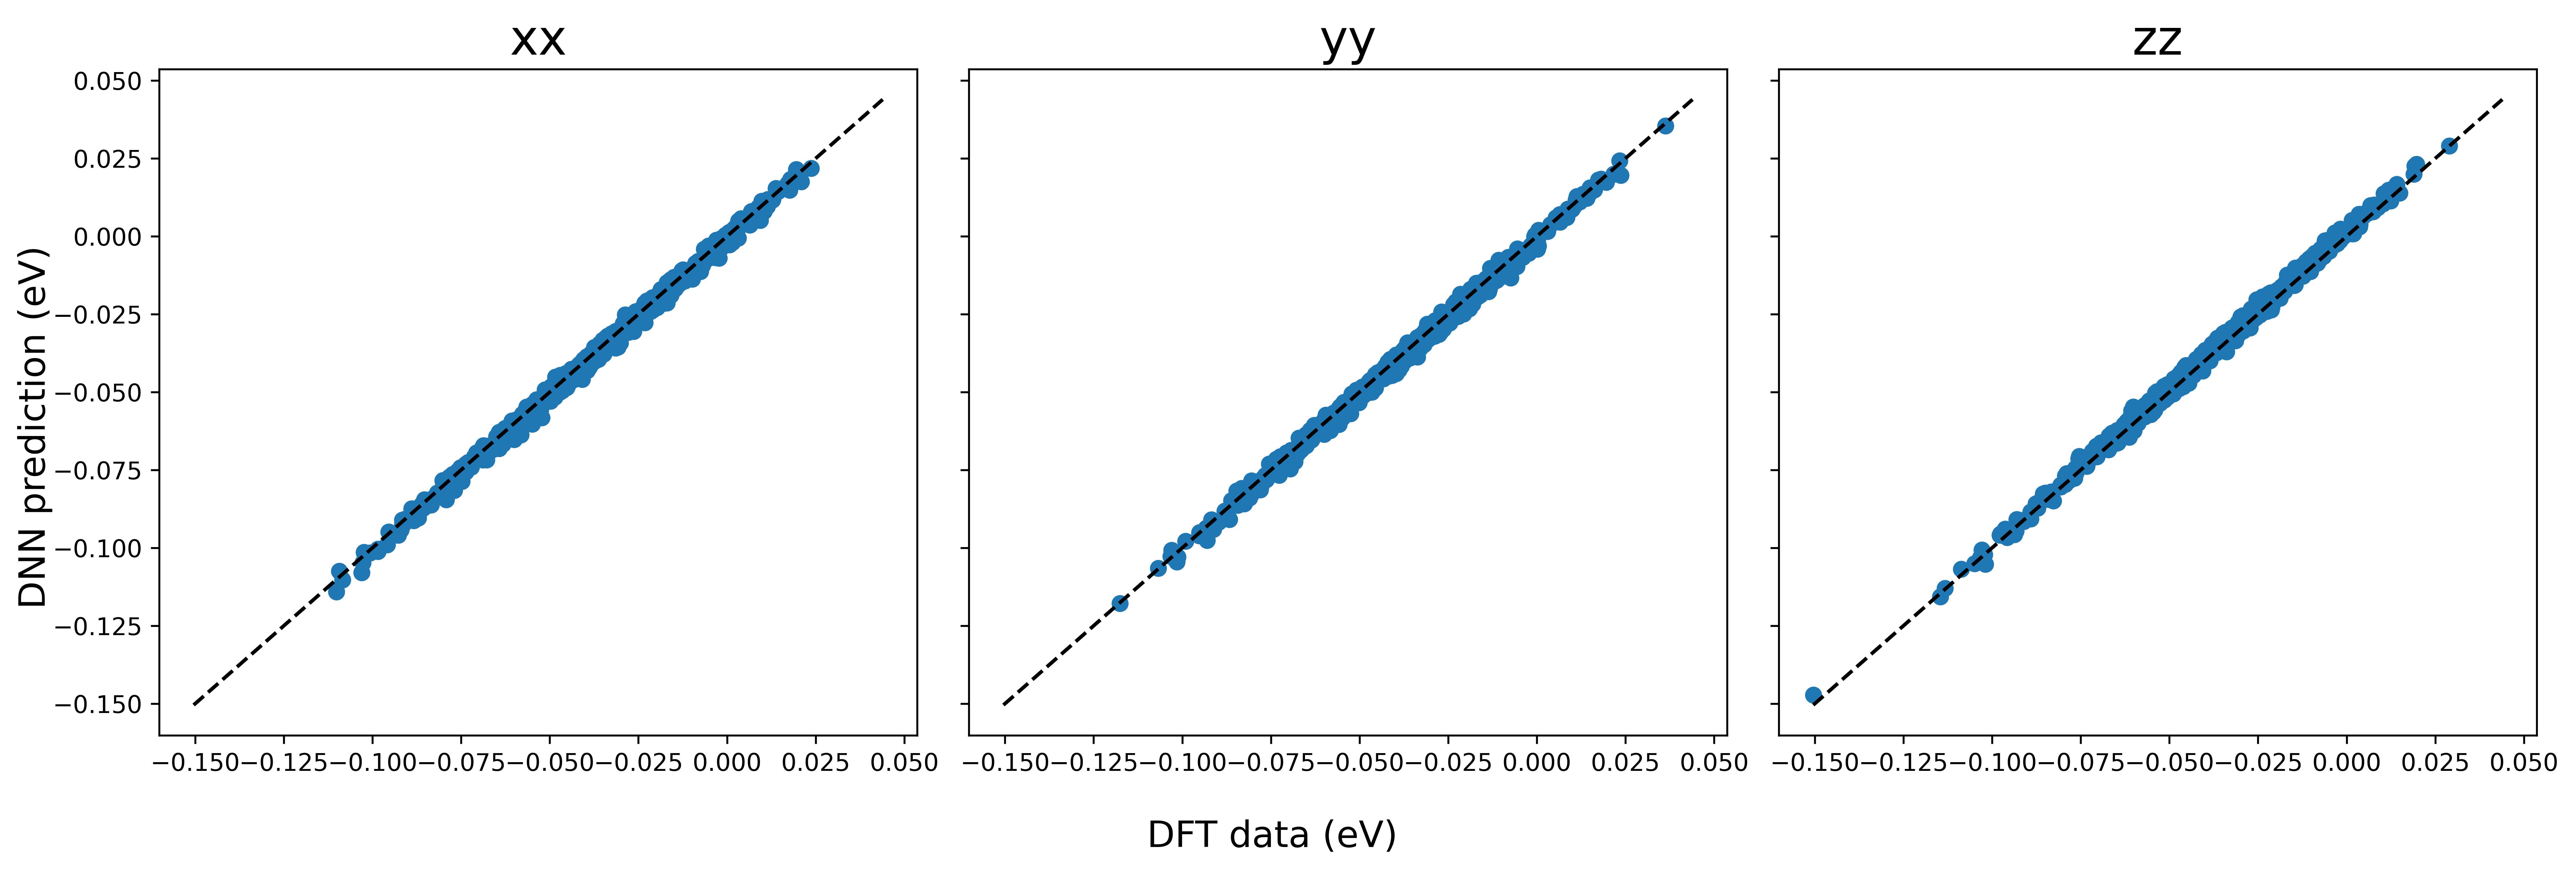
\includegraphics[width=0.9\textwidth]{images/bulk+interface_NN_on_interface/2_virial_peratom.png}
    \caption{Virial per atom}
    \label{fig:corr_bulk+interface_NN_P}
  \end{subfigure}
  \caption{Correlation between deep NN prediction data with the DFT data for
    a
    model trained on bulk and interface systems. The
    diagonal line shows the perfect agreement between the two data.}
  \label{fig:corr_bulk+interface_NN}
\end{figure}

\section{Density}

\begin{figure}[h!]
  \centering
  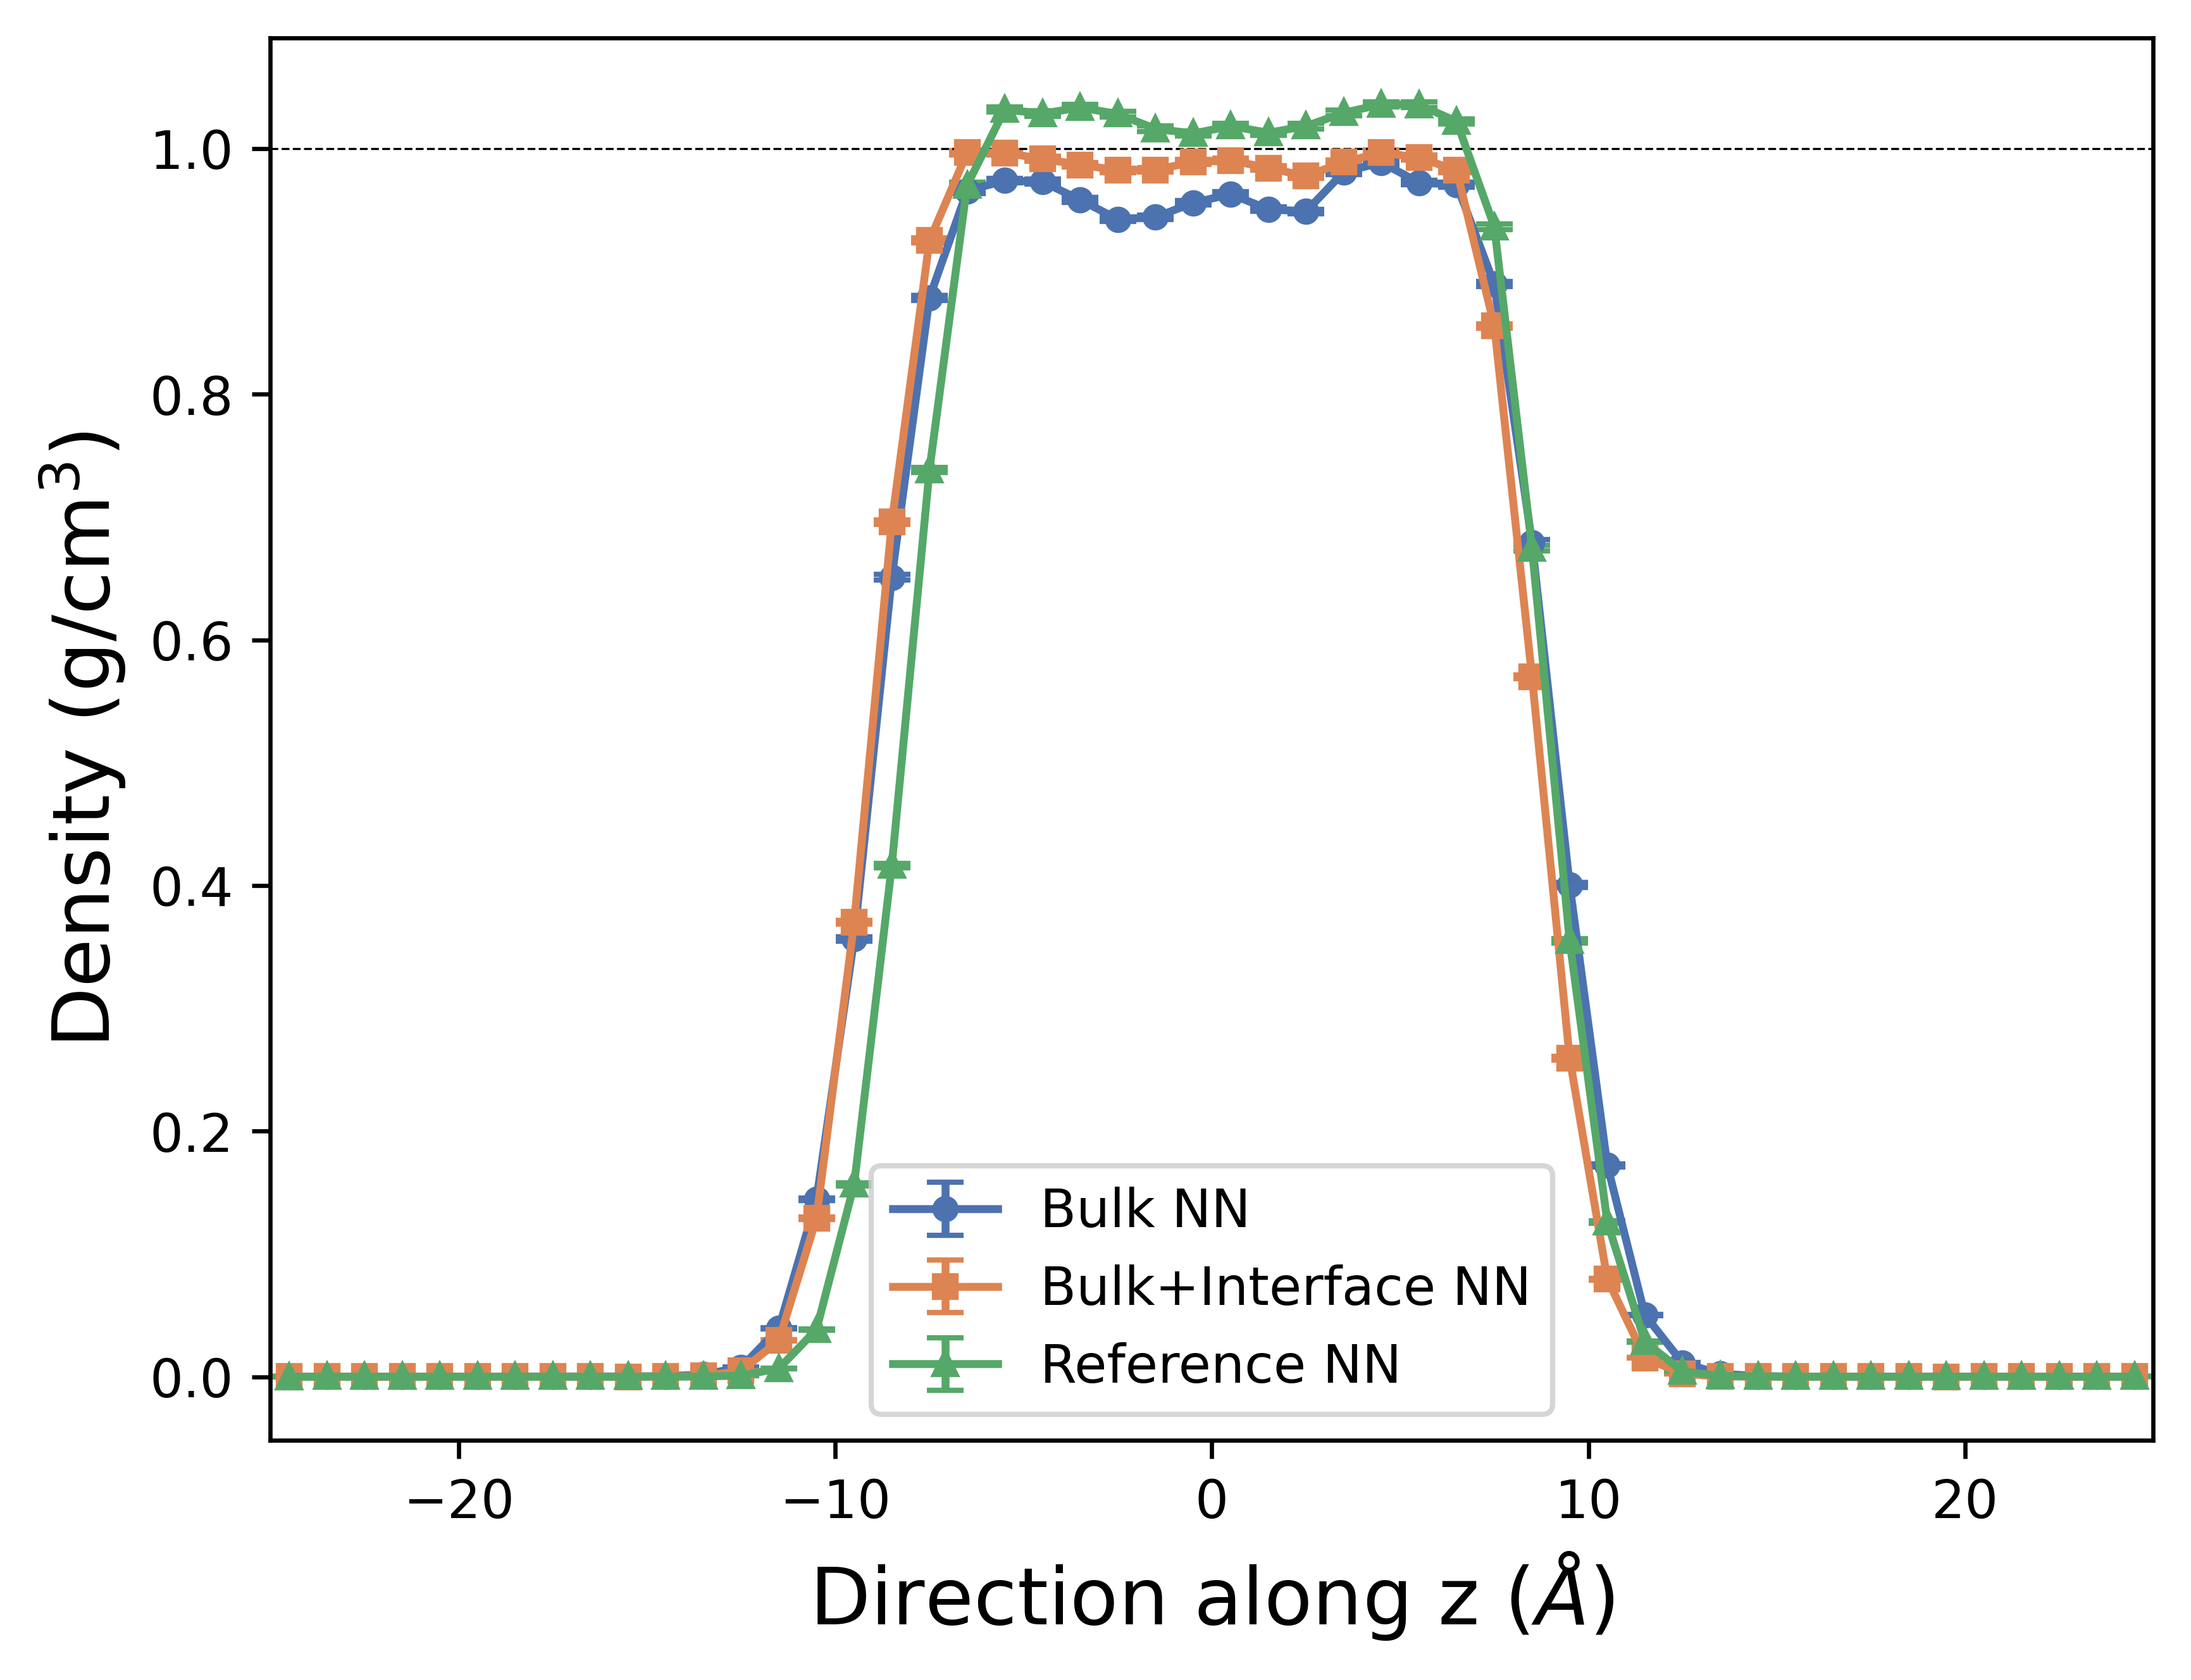
\includegraphics[width=0.7\linewidth]{images/density_330.png}
  \caption{Mass Density Profile at 330 K for different deep neural network
    models. The reference model is based on trained model of Sanchez-Burgos et
    al.~\cite{sanchez2023deep}. }
  \label{fig:density}
\end{figure}

\section{Surface Tension}
\begin{figure}[h!]
  \centering
  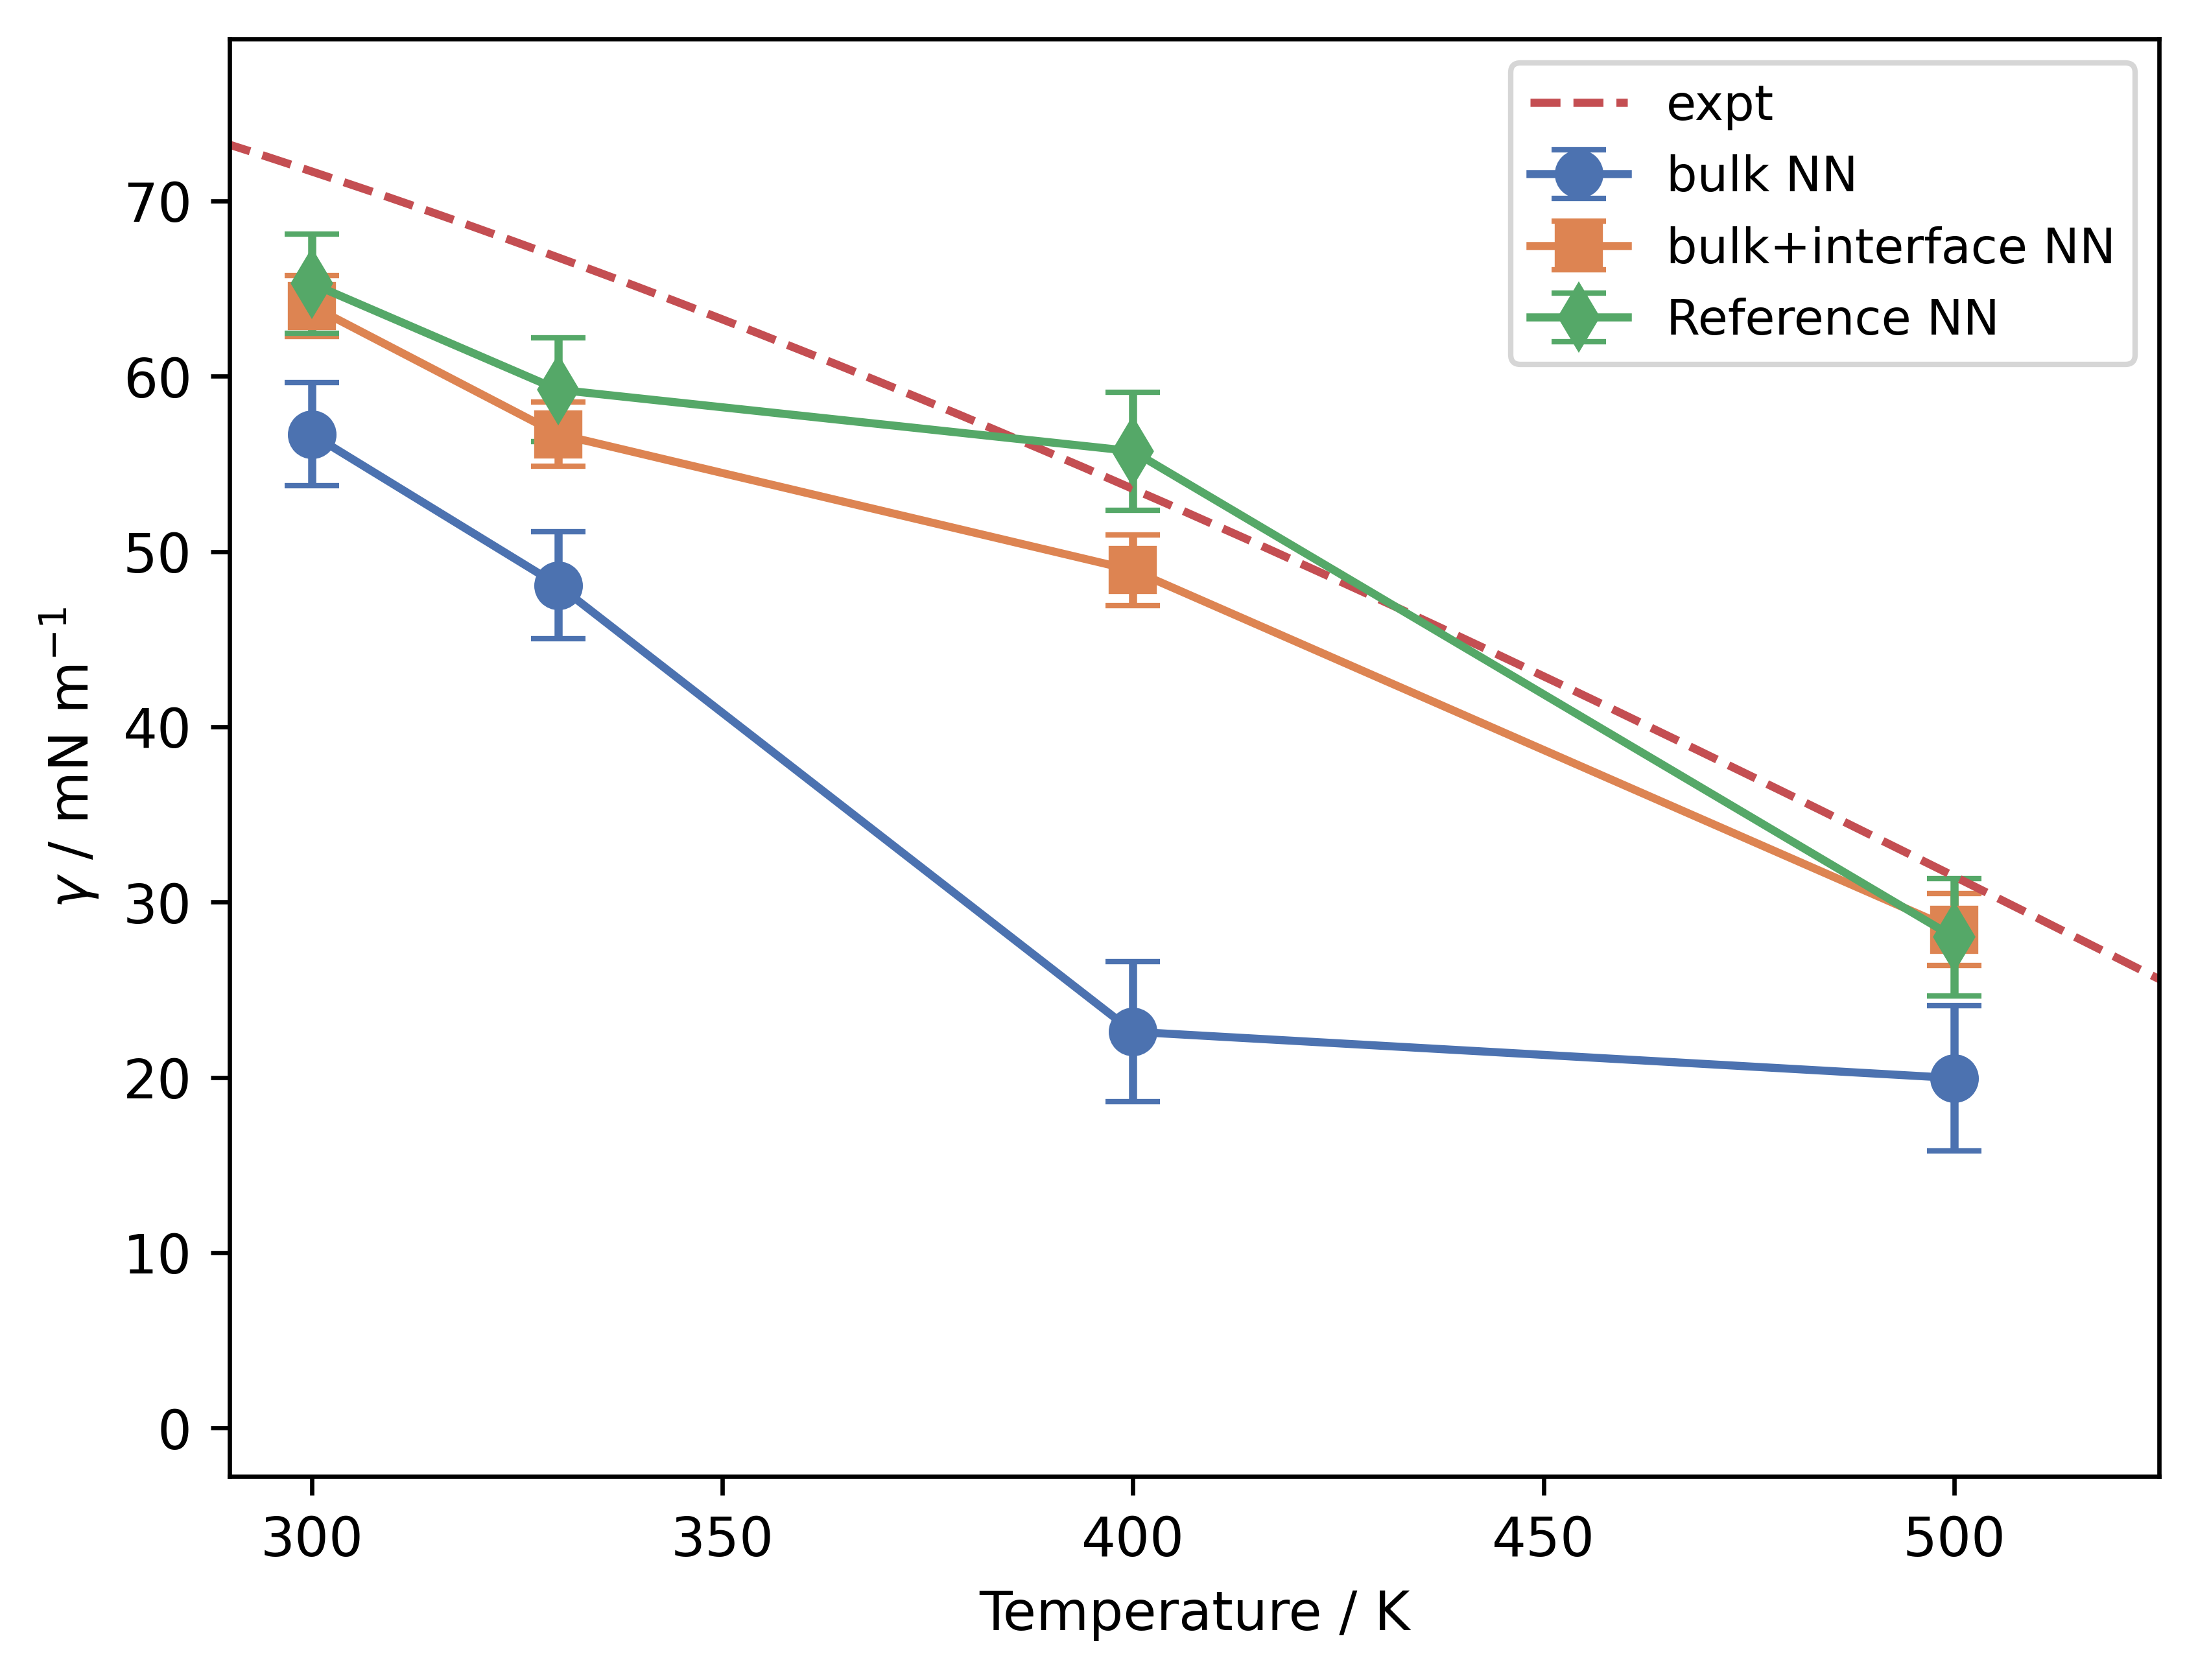
\includegraphics[width=0.7\linewidth]{images/surface_tension.png}
  \caption{Surface Tension}
\end{figure}
\begin{figure}[h!]
  \centering
  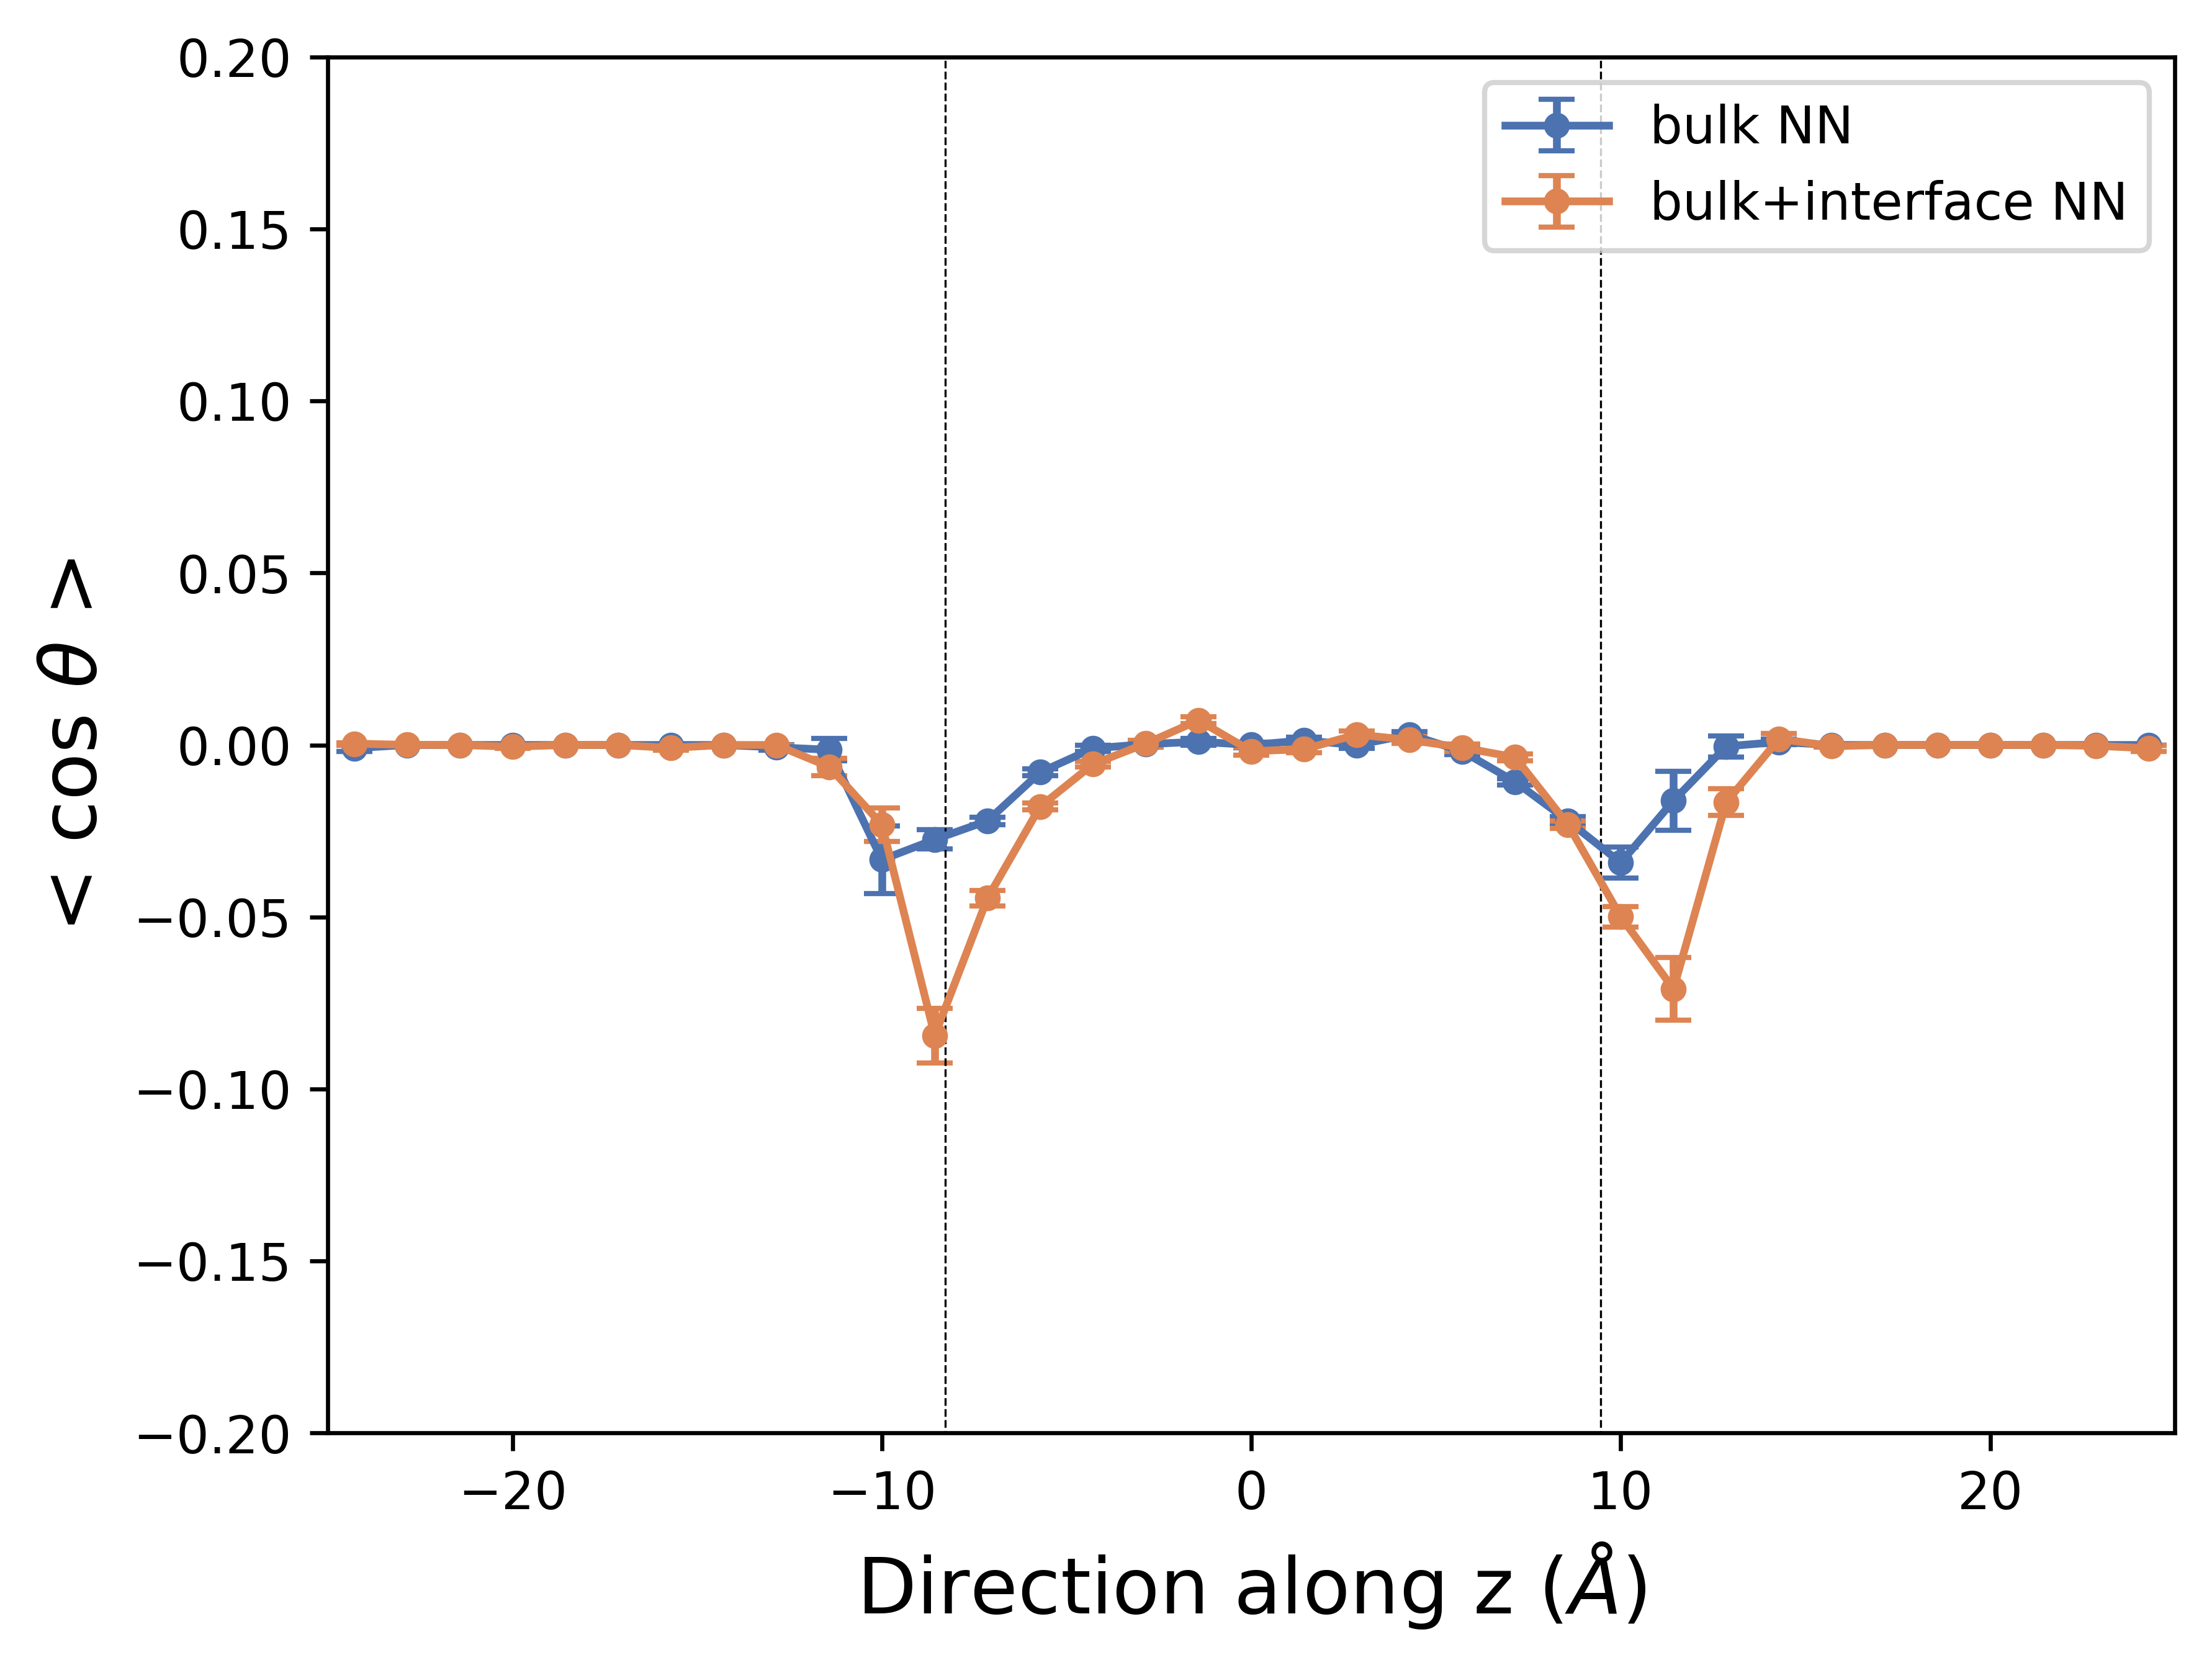
\includegraphics[width=0.5\linewidth]{images/dipole_dist.png}
  \caption{Dipole Orientation}
\end{figure}

\begin{figure}[h!]
  \centering
  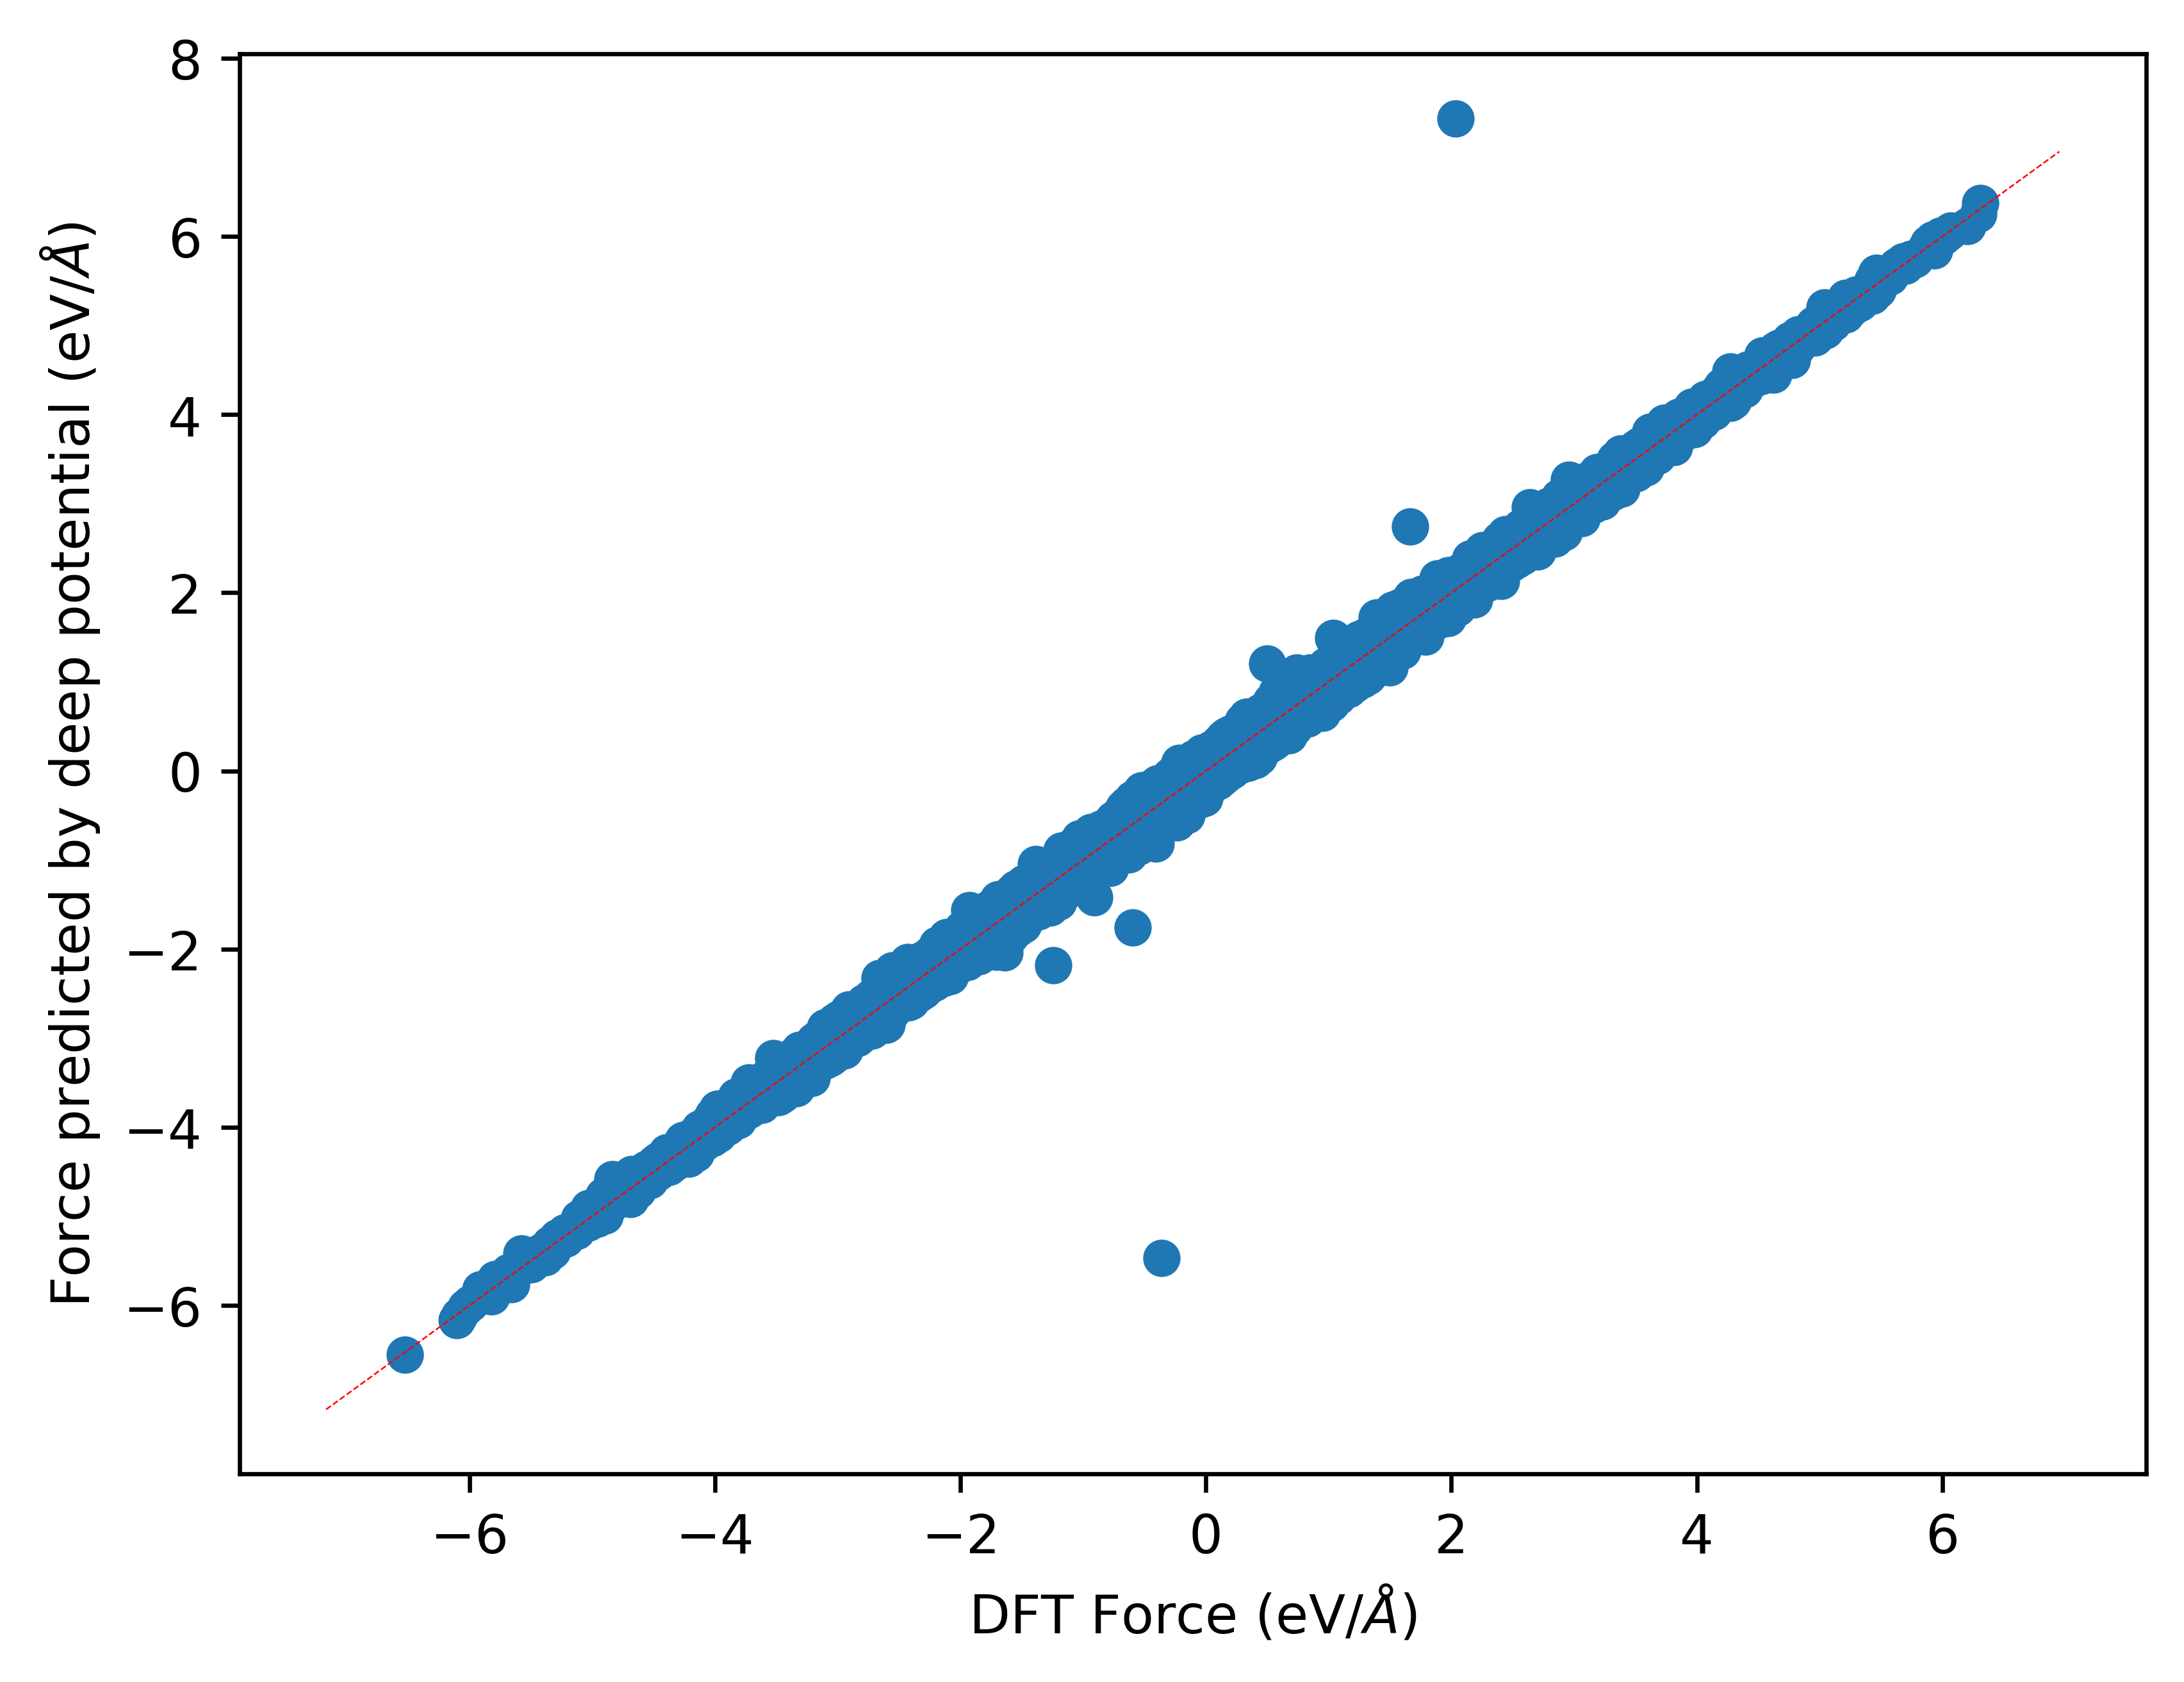
\includegraphics[width=0.5\linewidth]{images/force_correlation.png}
  \caption{Correlation between the predicted and reference data}
\end{figure}

\section{Dipole Orientation}
\section{Model Deviation}

\clearpage
